\part{Geophysical Fluid Dynamics}\label{Geophysical Fluid Dynamics}

\section*{Introduction}

This section of the course was lectured by \href{https://www.physics.ox.ac.uk/our-people/woollings}{Tim Woollings} covering Basic and Advanced Geophysical Fluid Dynamics (GFD). Basic GFD is covered in HT, while Advanced GFD is covered in Trinity term.\vspace{5 mm}

\noindent This section consists of six chapters. Basic GFD covers the first four chapters, and Advanced GFD covers the last two:\vspace{5 mm}

\begin{enumerate}
    \item \hyperref[Prelim GFD]{Preliminaries}: 
        
        \begin{quote}
            This chapter covers some preliminaries that are worth getting out of the way prior to 
        \end{quote}

    \item \hyperref[EoM GFD]{The Equations of Motion}: 
    
        \begin{quote}
            To be perfectly honest, you could skip almost all of the section except for the final coloured box should you wish. Here we introduce the primitive equations of motion governing the fluid mechanics of the atmospheres and oceans. We main aim of this chapter is to simplify the equations of motion blah blah balh
        \end{quote}
    
    \item \hyperref[Dia Relations]{The Fundamental Diagnostic Relations}:
        
        \begin{quote}
            We introduce some fundamental diagnostic (time-independent) relations, including hydrostatic balance and geostrophic balance, then discuss the implications on (anti-)cyclones and Thermal Wind Balance. We use hydrostatic balance to transform explicitly into pressure coordinates, and express the prior relations in terms of pressure coordinates.

            I should note that even though such relations are diagnostic (i.e., they feature no time-derivatives), it is worth considering that such relations might still hold even if the system is changing: in this case, the relations may hold in a quasi-steady manner (a concept introduced in Part \ref{Climate Dynamics}).
        \end{quote}
    
    \item \hyperref[Shallow Water System]{The Shallow Water System}:
        
        \begin{quote}
            We finally analyse a simple time-dependent system. In doing so, we sacrifice the vertical dimension (i.e., dispense of the vertical coordinate $z$) and work solely in a 2D system. We use this sytem to introduce energy in GFD, including KE (Kinetic Energy) and APE (Available Potential energy), as well as Potential Vorticity. Finally, we show that the (linearised) Shallow Water Systems allows certain wave solutions, including Poincaré, Kelvin, and Rossby Waves.
        \end{quote}
    
    \item \hyperref[3D Systems]{3D Systems}:
        
        \begin{quote}
            We reintroduce the vertical coordinate $z$ and analyse 3D GFD. After a brief stint looking at 3D Gravity Waves, we introduce Quasi-Geostrophic Theory. We then analyse Rossby Waves through this framework, then give a very cursory introduction to Instability and Geostrophic Turbulence.
        \end{quote}

    \item \hyperref[Oceans]{Ocean Circulation}:
        
        \begin{quote}
            The final section in GFD focuses exclusively on the Oceans. We first introduce Ekman Transport (which is applicable to the Atmosphere, in its own right). We then analyse the implications of such transport, including Sverdrup Balance. Finally, we briefly discuss the Meridional Overturning Circulation, and introduce two simple models which aim to capture the dynamics: the Stommel and Gnanadesikan Box Models.
        \end{quote}
\end{enumerate}

\chapter{Preliminaries}\label{Prelim GFD}

\section{A Quick Reminder on Vector Calculus}

Before we jump into \textbf{Geophysical Fluid Dynamics} (\textbf{GFD}) proper, we start with a quick reminder of some concepts in vector calculus. I'll mainly focus on the interpretation of certain concepts, as this will be important for the interpretation of physical results later on.

You should be familiar with all the information in the box below:

\begin{fact}{Vector Calculus Definitions}{VC box}\label{VC box}
    Let $\vec{r}=(x,y,z)^T$ denote the position vector and $t$ denote the time.\vspace{3mm}

    \begin{minipage}{0.49\linewidth}
        We write the \textbf{partial derivative} of coordinate $x_1$ as follows (the subscripts indicate which variables are held constant while differentiating; in this case, coordinates $x_2, \, x_3,\, t$ are held constant while differentiating $x_1$):
        \begin{align}\label{partial}
            \partial_{x_1}=\frac{\partial}{\partial x_1}=\left( \frac{\partial}{\partial x_1} \right)_{x_2,\,x_3,\,t}
        \end{align}
        Often we will omit the large brackets and leave implicit which coordinates are being held constant.
    \end{minipage}
    \hfill
    \begin{minipage}{0.49\linewidth}
        We define the \textbf{nabla} operator $\vec{\nabla}$ as follows (in Cartesian coordinates):
        \begin{align}
            \vec{\nabla}&=\left( \begin{array}{c}
                \frac{\partial}{\partial x}\\\\
                \frac{\partial}{\partial y}\\\\
                \frac{\partial}{\partial z}
            \end{array} \right)
            \\
            &=\left( \frac{\partial}{\partial x}, \frac{\partial}{\partial y}, \frac{\partial}{\partial z} \right)^T \nonumber
        \end{align}
    \end{minipage}

    \vspace{3mm}Let $p(\vec{r},t)$ be an arbitrary scalar field and $\vec{u}(\vec{r},t)=(u_x,u_y,u_z)^T$ be an arbitrary vector field.

    We define the \textbf{Gradient}, \textbf{Curl}, and \textbf{Divergence} as follows:

    \begin{minipage}{.44\linewidth}
        \begin{align}
            \BOX{\text{Grad}\,\, p \equiv \vec{\nabla}p=\left( \begin{array}{c}
                \frac{\partial p}{\partial x}\\\\
                \frac{\partial p}{\partial y}\\\\
                \frac{\partial p}{\partial z}\\
            \end{array} \right)}
        \end{align}
    \end{minipage}
    \hfill
    \begin{minipage}{.54\linewidth}
        \begin{align}
            \BOX{\text{Curl}\,\, \vec{u} \equiv \vec{\nabla}\times \vec{u}=\left( \begin{array}{c}
                \frac{\partial u_z}{\partial y}-\frac{\partial u_y}{\partial z}\\\\
                \frac{\partial u_x}{\partial z}-\frac{\partial u_z}{\partial x}\\\\
                \frac{\partial u_y}{\partial x}-\frac{\partial u_x}{\partial y}\\
            \end{array} \right)}
        \end{align}
    \end{minipage}

    \begin{align}
            \BOX{\text{Div}\,\, \vec{u} \equiv \vec{\nabla}\cdot \vec{u}= \frac{\partial u_x}{\partial x} + \frac{\partial u_y}{\partial y} + \frac{\partial u_z}{\partial z}}
    \end{align}


\end{fact}

In this box we mentioned a \textbf{scalar field} and \textbf{vector field}. A field is just anything that has a value at each point in space and time. There are two kinds you will need to know: a \textbf{scalar field} and a \textbf{vector field}. A \textbf{scalar field} is a field that takes a scalar value at each point. For example, the pressure field $p=p(\vec{r},t)$ is a scalar field, which denotes the pressure at each point in space/time. Meanwhile, a \textbf{vector field} is a field that takes a vector value at each point. For example, the velocity field $\vec{u}=\vec{u}(\vec{r},t)$ is a vector field, which denotes the velocity at each point in space/time. While what I'm about to say isn't strictly correct, you can just think of a vector field as three scalar fields stacked on top of each other (one for each component).

Now we will interpret in turn the \textbf{Gradient}, the \textbf{Curl}, and the \textbf{Divergence}.

\subsection{The Gradient}

We can only take the gradient of a \textbf{scalar field} and the the gradient of a field is always a \textbf{vector field}.

The gradient encodes the local change properties of the \textbf{scalar field}. More specifically, at each point in space and time, the value of the gradient is a vector with the following properties: the direction (in 3D space) of the vector is in the direction of steepest ascent, and the magnitude of the vector denotes how much the scalar field ascends at that point.

You should be familiar with the one-dimensional Taylor Expansions. Consider some function $f: \mathbb{R} \to \mathbb{R}$\footnote{This is fancy speak for the function $f(x)$ takes real numbers as an input and outputs real numbers.}. The following holds expresses the Taylor expansion, which holds for small $\delta x$:
\begin{align*}
    f(x+\delta x)=f(x)+\frac{df}{dx}\delta x
\end{align*}
An analogous version holds in three dimensions as well:
\begin{align*}
    p(\vec{r}+\delta\vec{r},t)&=p(\vec{r},t)+\left( \vec{\nabla}p(\vec{r},t) \right)\cdot \delta\vec{r}\\
    &=p(\vec{r},t)+\left( \text{Grad }p(\vec{r},t) \right)\cdot \delta\vec{r}
\end{align*}

Consider the case where $\delta \vec{r}$ is perpendicular to $\vec{\nabla}p$ (i.e., $\vec{\nabla}p\cdot \delta \vec{r}=0$). In this direction, there is no local change in $p$, therefore $p(\vec{r}+\delta\vec{r},t)=p(\vec{r},t)$ for all $\delta\vec{r}\perp \vec{\nabla}p$. This implies that contours of constant $p$ are \textbf{always} perpendicular to the gradient of $p$. 

\subsection{The Curl}

We can only take the curl of a \textbf{vector field}, a field that take a vector at each point in space. The curl is always a \textbf{vector field}.

Broadly, the curl measures the local rotation of the \textbf{vector field}. More specifically, at each point in space and time, the value of the curl is a vector with the following properties: the direction (in 3D space) of the vector is in the direction perpendicular to the plain of rotation (following the right-hand rule)\footnote{This is simply a convention. The right hand rule means that if you form a thumbs up with your right hand, your thumb is parallel with the vector if and only if the rotation is in the direction from your knuckles to the end of your fingers (following your fingers).}, and the magnitude of the vector denotes how much local rotation there is at this point.

Note crucially that this only measures the \textbf{local} rotation, not the global rotation. The example often given to explain this distinction is a paddleboard: consider a 

\subsection{The Divergence}

We can only take the divergence of a \textbf{vector field}, a field that takes a vector value at each point in space. The divergence is always a \textbf{scalar field}.

Broadly, the divergence measures the local `spreading out' properties of a \textbf{vector field}. More specifically, at each point in space and time, the value of the divergence is a scalar that is larger the more 

I find the divergence theorem to explain divergence the easiest:
\begin{align}
    \label{Div Thm}
    \iiint_v \vec{\nabla}\cdot \vec{u} \,dV \equiv \iint_s \vec{u}\cdot d\vec{S}
\end{align}
where $v$ and $s$ denote that we integrate over the volume and surface, respectively, of some closed 3D blob (closed means there are no holes on the blob). Suppose that $\vec{u}$ is some flux per unit area. If, for example, $\vec{u}$ is the velocity, then $\vec{u}$ would be the volume flux per unit area. 

The divergence theorem says that the \textit{total flux} out of some blob (equal to the integral of $\vec{u}$ over the surface of the blob, i.e., the right-hand side of \ref{Div Thm}) is equal to the \textit{total divergence} of the blob (equal to the integral of $\vec{\nabla}\cdot\vec{u}$ over the volume of the blob, i.e., the left-hand side of \ref{Div Thm}). 

The divergence can therefore be thought of as the outwards flux of $\vec{u}$ at some point, i.e., as encoding how many vectors point towards or away from a point. If the divergence is positive/negative, more/less arrows point outward than inward at that point (respectively). If the divergence is $0$, then exactly the same `amount' of arrows point inwards as outwards. 

As a summary:
\begin{fact}{Vector Calculus Interpretation}{VC Interp}\label{VC Interp}
    The gradient blah blah blah
\end{fact}

\section{A Quick Reminder of Fluid Mechanics}

To aid understanding, we quickly introduce some concepts of fluid mechanics. Tim should have a more comprehensive review on canvas should you need it.

First we introduce the concept of a fluid element. This is an infinitesimal volume of fluid, whose properties may change as it is advected around with the flow. For example, in deriving the \hyperref[Dry Adiabat]{Dry Adiabat}, we were considering a fluid element of air – except we called it an `air parcel' then.

Second, we introduce the \hyperref[Material Derivative]{Material Derivative}:
\begin{align}
    \frac{D}{Dt}=\underbrace{\frac{\partial}{\partial t}}_{\text{Time Derivative at a Fixed Point}}+\underbrace{\vec{u}\cdot\vec{\nabla}}_{\text{Advection}}
    \label{Material Derivative}
\end{align}
The \hyperref[Material Derivative]{Material Derivative} of a quantity is the time-derivative of a quantity \textit{following a fluid element}. This is useful because it is much easier to consider what effects might change a quantity of a fluid element. For example, the forces per unit mass $\vec{F}$ affect a fluid parcel as follows: $\frac{D\vec{u}}{Dt}=\vec{F}$ (this is just Newton's second law).

However, in GFD, we will mostly be interested in how a quantity changes at a \textbf{fixed point in space} $\left(\text{indicated by the } \frac{\partial}{\partial t} \text{ term}\right)$, \textit{not following a fluid element}. If we rearrange the Equation \ref{Material Derivative} for $\left( \frac{\partial}{\partial t} \right)$, we find that the quantity at some point is modified by both whatever affects the fluid element $\left( \frac{D}{D t} \right)$, for example the force $\vec{F}$, and the properties of fluid elements which are advected into that location $-\vec{u}\cdot\vec{\nabla}$:
\begin{align}\label{MatDerivTerms}
    \underbrace{\frac{\partial A}{\partial t}}_{\text{Local change in }A}=
    \underbrace{\frac{DA}{Dt}}_{{\text{Change in }A \text{ following a fluid element}}}-
    \underbrace{\vec{u}\cdot\vec{\nabla}A}_{\text{Advection of fluid elements with different }A}
\end{align}

Hopefully you can see why this physically makes sense. The local change in $A$ is the is comprised of the the change in $A$ following a fluid element, i.e., comprised of what happens exactly at that point, \textbf{and} advection, i.e., the effect of fluid elements that low into that point. Advection is the negative dot product of $\vec{u}$ with the gradient of $A$. Hopefully this makes sense too: the gradient points in the direction of increasing $A$. If $A$ is increasing in the same direction as $\vec{u}$, then $\vec{u}$ is `blowing' areas of lower $A$ into areas of higher $A$, so this should be a negative contribution to the local change in $A$.

Third, we introduce the idea of \hyperref[Material Conservation]{Material Conservation}. You might have heard about what it means for a quantity to be \textbf{conserved}. For example, if you've solved a mechanics problem, you might recall that the total energy was conserved, meaning that $\frac{dE}{dt}=0$ where $E=$ the total energy.

\hyperref[Material Conservation]{Material Conservation} is a closely related idea, where certain quantities are conserved following a fluid parcel. Mathematically, a quantity $A$ is materially conserved if and only if it obeys the following relation:
\begin{align}\label{Material Conservation}
    \frac{D A}{Dt }=0
\end{align}
In other words, if one follows a fluid parcel, that quantity does not change. However, as a whole, $A$, need not be globally conserved. If one considers Equation \ref{MatDerivTerms} and sets $\frac{D A}{Dt }=0$, then you can see that the only local change in $A$ is from fluid parcels with different $A$ being advected into that location.

Exercise: refer forwards to Equation \ref{Energy Equation}. Note even if we assume that $Q=0$, we will find that $\frac{DT}{Dt}\neq 0$. In other words, temperature is not materially conserved (so long as $\beta\neq0$). This is why we introduced the idea of \hyperref[Potential Temperature]{Potential Temperature}, as it is the case that $\frac{D\theta}{Dt}=0$ (excercise: take \ref{Energy Equation}, solve for $\beta$ using the ideal gas law, set $Q=0$, and show that $\frac{D\theta}{Dt}=0$ using the product rule).

Finally, we define the vorticity $\vec{\omega}$ as the curl of the velocity:
\begin{align}
    \vec{\omega}=\vec{\nabla}\times\vec{u}
\end{align}
If you refer back to the box on \hyperref[VC Interp]{Vector Calculus Interpretation}, this should remind you that the curl of the velocity is the \textbf{local} rotation of the velocity field, not the \textbf{global} rotation. We will usually be considering the vertical component of the vorticity $[\vec{\omega}]_z$, which we will often write just as $\xi$.

\section{Why There Is Motion in the First Place}

It's important to consider why there is motion in Atmospheres and Ocean in the first place.

Regarding the first point, if you are familiar with the \hyperref[Navier Stokes]{Navier Stokes Equations} governing fluid flow, then you will know that $\vec{u}=\vec{\nabla}p=0$ is a solution, and is a solution a system will tend towards if there is friction and forcing\footnote{This forcing can be encoded in the boundary conditions, for example.}, and planets certainly have friction. We therefore need a non-uniform energy source. In this case, it is the Sun, and it drives motion because it provides energy to the Earth unevenly. On small scales, this may be because of variations in reflectivity (albedo), but on large scales this is mostly due to the spherical geometry of the Earth: more solar radiation is absorbed at the equator than at the poles (think: \textbf{zenith angle} from \hyperref[Radiative Transfer]{Radiative Transfer}, which goes as $\cos\zeta$).

This differential heating causes horizontal temperature gradients, which in turn cause horizontal density and pressure gradients, which drive motion. Another way to think of it is as follows: in equilibrium, the Earth absorbs more solar radiation in the equator than in the poles (see Figure \ref{Diff Heating}). As such, there must be an energy transport mechanism from the equator to the poles, and this is what drives fluid motion.\footnote{
    I'm personally somewhat ambivalent about this explanation, but I'm not very confident so be sceptical of what I'm about to say. Here's why I'm uncomfortable about this explanation: I cannot see why it must be the case that the variation in OLR cannot be identical to the variation in absorbed solar radiation. To put it another way, I cannot see why the dotted curve cannot be identical to the solid curve in Figure \ref{Diff Heating}. It feels like putting the cart before the horse: surely the fluid dynamics also itself affects the OLR into space.

    I prefer the following explanation. Assume that differential heating did not obtain, and that the poles and equator were in perfect equilibrium, such that the absorbed solar at each point exaclty equalled the OLR. Because the absorbed solar is more at the equator than the poles, that means the OLR must be more at the equator than the poles. Loosely following the properties of emission (recall  \hyperref[Emission Box]{this information on emission}) suggests that the poles must be colder than the poles. 

    This implies that there must be horizontal temperature gradients, and where there are temperature gradients there are density gradients. These horizontal density gradients generate instability, because a system with the minimum amount of gravitational potential energy will only have \textit{vertical} density gradients: hence motion.
}

\begin{figure}[H]
    \centering
    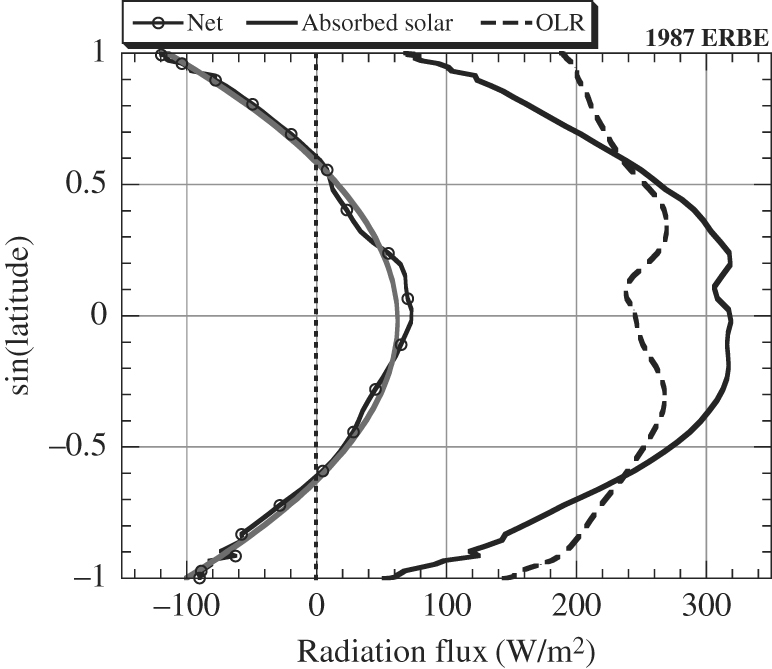
\includegraphics[width=0.5\linewidth]{Figures/GFD/Diff Heating.jpg}
    \caption{Figure from Ray's book showing differential heating. More heat is }
    \label{Diff Heating}
\end{figure}



\section{What is Special About `Geophysical' Fluid Mechanics?}\label{GFD Special}

It is also important to consider what sets \textbf{Geophysical Fluid Dynamics} apart from most other Fluid Dynamics. There are two important properties that \textbf{Geophysical Fluid Dynamics} aim to investigate: \textbf{stratification} and \textbf{rotation}. The effects of these will pop up again and again throughout \hyperref[Geophysical Fluid Dynamics]{GFD}.

\subsection{Stratification}

\textbf{Stratification} is important because the fluids in the atmospheres and oceans are affected by gravity and vary in density. 

You have already seen the effect of stratification when we derived the \hyperref[Hydrostatic Balance]{Hydrostatic Balance}. We found that pressure decreases with height 
\begin{align*}
    \frac{dp}{dz}=-\rho g\\
    \frac{d}{dz}\left( \rho R T \right)=-\rho g\\
    RT \frac{d \rho}{dz} + \frac{}{}
\end{align*}

REFER TO THE BUOYANCY FREQUENCY SECTION IN THE CLOUDS SECTION

\subsection{Rotation}

\textbf{Rotation} is important because, generally, planets rotate, and the equations of motion ensure that fluid parcels must obey conservation of angular momentum. The idea is as follows: if a fluid parcel is at rest relative to the surface of the Earth, its total angular momentum will actually differ depending on where it is. If it is at the poles, it will have no angular momentum, whereas if it is at the equator, it will have a large amount of angular momentum.

In the previous section, we discussed how differential heating implies that there must be some motion. This motion is required to close the energy budget. Becuase there both is net radiative heating at the equator and net radiative cooling at the poles, and the equator and poles are not heating and cooling over time, there must be some mechanism transfering energy from the equator to the poles. This is achieved by the atmospheres and oceans.

Let us then consider a extremely simple model of this: \textbf{Hadley's Model} of convection as a zonally (zonally means east-west) symmetric equator-to-pole convection cell:
\begin{figure}[H]
    \centering
    \begin{tikzpicture}
        \draw (0,0) -- (5,0) arc[start angle=0, end angle=90, radius=5cm] -- cycle;
        %\draw (5,0) -- (0,0) -- (0,5);
        \draw (0,0) -- (3,0) arc[start angle=0, end angle=90, radius=3cm] -- cycle;
        %\draw (3,0) -- (0,0) -- (0,3);
    \end{tikzpicture}
    \caption{Convection Cell}
\end{figure}

Let us not consider a fluid parcel in this convection cell. We assume that this fluid parcel starts out at the equator at rest (relative to the surface of the Earth) and moves north. We also assume that there are no zonal forces (i.e., no east-west forces) acting on the fluid parcel. This is a highly unrealistic assumption. We further assume that the radius of the Earth $a$ is much larger than the height of the fluid parcel above the Earth.

We know that the total angular momentum of the parcel is approximately equal to the following:
\begin{align*}
    L(\phi,u) = \underbrace{a\cos\phi}_{\vec{r}} \underbrace{\left( \Omega a \cos \phi + u \right)}_{\vec{u}}
\end{align*}
where $a=$ the radius of the Earth, $\phi=$ the latitude, $\Omega=$ the angular velocity of the Earth, and $u=$ the zonal velocity of the fluid parcel relative to the surface of the Earth. The angular momentum is equal to $\vec{r}\times\vec{u}$, the radius $\vec{r}$ times the velocity $\vec{u}$. The radius is equal to $a\cos\phi$ (as it is the radius from the axis of rotation), and the velocity is equal to $\Omega a \cos \phi + u$, the sum of the velocity from the rotation of the Earth and the velocity relative to the Earth.\footnote{
    This is, strictly speaking, incorrect. The angular momentum is a vector (actually a pseudo-vector), so it’s strange to say that the angular momentum is equal to a scalar value. To be more precise, $L(\phi,u)$ is the component of the angular momentum in the direction aligned with the angular velocity of the Earth. In other words parallel the vector pointing directly upwards from the ground at the north pole.
}

Since there are no zonal forces on the air parcel, this implies that the angular momentum is conserved. Setting $L(\phi,u)=const$ imposes the constraint $u=u(\phi)$. We use our assumption that, at $\phi=0$ (the equator), the $u=0$ (fluid parcel is at rest). Therefore, some simple algebra gives us the following relation:
\begin{align*}
    \boxed{u=a\Omega \left( \frac{1}{\cos\phi}-\cos\phi
    \right)}
\end{align*}

Essentially, what this says is that, as the air parcel moves north (as $\phi$ increases), the zonal velocity $u$ also increases! Conservation of angular velocity imposes that the air parcel is deflected as it moves northwards, so fluid parcel motion cannot always be as straightforward on a rotating planet as on a non-rotating planet.

Of course, this model is highly unrealistic. Firstly, it predicts that $u\to\infty$ at $\cos\phi\to\pi/2$, which is clearly unphysical. Secondly, from observations, we pretty much never observe $u\geq\qty{150}{\metre\per\second}$, so the model fails much earlier than $u\to\infty$. In reality, our assumption that there were no zonal forces was a very inaccurate assumption: as horizontal velocities become arbitrarily large, these induce large shears (a shear is when a layer of stuff (e.g., air) is sliding over another layer of stuff (e.g., air)), which in turn induce large forces either from viscous or turbulent eddy stresses.\footnote{For a cursory look at the effect of vertical stresses, refer to this section on \hyperref[Ekman Transport]{Ekman Transport}!}

However, the general moral of the story does apply: there are conservation laws that constrain motion more on rotating planets than non-rotating planets. We find that this will actually be the Material Conservation of Potential Vorticity, but this is jumping ahead a bit.

Looking back, this should be seen as as cursory, highly unrealistic taste of the effect that stratification and rotation might have on dynamics. It won't be much of an exaggeration ot say that we'll spend most of GFD discussing the effects of rotation.

\chapter{The Equations of Motion}\label{EoM GFD}

\section{The Primitive Equations of Motion}

For simplicity we ignore state variables like salinity, humidity, etc., and restrict our attention to a system fully characterised by 6-state variables: the velocity $\vec{u}=(u,v,w)$, pressure $p$, density $\rho$, and temperature $T$. These are governed by six equations: 3 momentum budget equations (\ref{Navier Stokes}), one mass budget equation (\ref{Mass Conservation}), one energy budget equation (\ref{Energy Equation}), and an equation of state (\ref{EoS}). Each term is labelled below:
\begin{gather}
    \boxed{\underbrace{\frac{D\vec{u}}{Dt}}_{\text{Acceleration and Advection}}
    =\overbrace{-\frac{1}{\rho}\vec{\nabla}p}^\text{Pressure Gradients}\underbrace{-g\vec{k}}_\text{Gravity}+\overbrace{\nu\vec{\nabla}^2\vec{u}}^\text{Viscous Dissipation}\underbrace{+\frac{\nu}{3}\vec{\nabla}(\vec{\nabla}\cdot\vec{u})}_\text{}+\overbrace{\vec{F}}^\text{Other Forces}}
    \label{Navier Stokes}
    \\
    \boxed{\underbrace{\frac{D\rho}{Dt}}_\text{Change in Mass of Fluid Parcel}\overbrace{+\rho\vec{\nabla}\cdot\vec{u}}^\text{Convergence/Divergence of Mass}=0}
    \label{Mass Conservation}
    \\
    \boxed{c_p\frac{DT}{Dt}-\frac{\beta T}{\rho}\frac{Dp}{Dt}=Q}
    \label{Energy Equation}
    \\
    \boxed{\rho=\rho(T,p,\ldots)}
    \label{EoS}
\end{gather}

\noindent where $\frac{D}{Dt}=\frac{\partial}{\partial t}+\vec{u}\cdot\vec{\nabla}$ is the material derivative; $g=$ gravitational acceleration; $\vec{k}=$ unit vector towards the centre of the Earth; $\nu=$ kinematic viscocity; $\vec{F}=$ other forces per unit mass (e.g., friction); $c_p=$ heat capacity per unit mass; $\beta=-\frac{1}{\rho}\frac{\partial \rho}{\partial T}$ thermal expansion coefficient; and $Q=$ heating per unit mass.

However, the equations currently are not fit for purpose. First, these equations are written for a coordinate system that is \textit{inertial} (non-accelerating) and \textit{cartesian}. However, the surface of the Earth is curved and the Earth is rotating\footnote{or so NASA and the lizard overlords would have you think!}, and we wish to describe what is going on \textit{here} with us. Furthermore, it would be quite demanding (computationally and conceptually) to adopt an inertial non-curved coordinate system, as then you'd have to, for example, keep track of the fact that the mountains keep moving. 

Second, these equations are currently too complicated to be analytically tractable. We will make various approximations later to simplify the equations of motion, however we should note that many of the terms we neglect cannot be neglected in a weather forecast or climate model.

\section{Simplifications}

\subsection{Rotating Coordinate Systems}

As already mentioned, the momentum budget equation applies for an \textit{inertial coordinate system}, i.e., a coordinate system which is not accelerating. However we wish to describe the dynamics in a rotating coordinate system which rotates with the Earth (or planet). Our goal now is to  find a relation between the time derivative of some arbitrary vector $\vec{A}$ in an inertial coordinate system $\left(\frac{d\vec{A}}{dt}\right)_I$ and the time derivative in a rotating coordinate system $\left(\frac{d\vec{A}}{dt}\right)$.

We consider two coordinate systems: an \textit{inertial} coordinate system and a \textit{rotating} coordinate system. Both systems share an origin, but the \textit{inertial} coordinate system rotates with a constant angular velocity $\vec{\Omega}$ where $|\vec{\Omega}|$ is the angular speed (in \qty{}{\radian\per\second}) and $\vec{\Omega}$ points along the axis of rotation.

Now consider some arbitrary vector $\vec{A}(t)$ in or rotating coordinate system. The time derivative in the inertial coordinate system $\left(\frac{d\vec{A}}{dt}\right)_I$ is related to the time derivative in the rotating coordinate system $\left(\frac{d\vec{A}}{dt}\right)_R$ as follows (see Figure \ref{Inertial to Rotating}):
\begin{figure}[H]
    \centering
    \begin{subfigure}{0.45\linewidth}
        \centering
        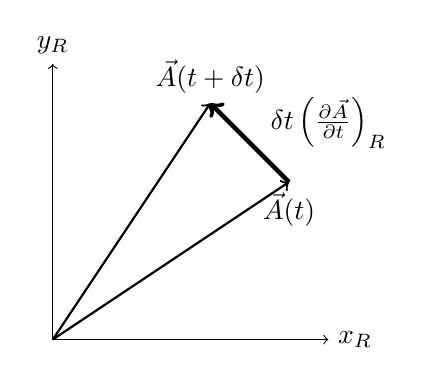
\begin{tikzpicture}
            \draw[->] (0,0) -- (3.5,0) node[anchor=west] {$x_R$};
            \draw[->] (0,0) -- (0,3.5) node[anchor=south] {$y_R$};
            \draw[thick,->] (0,0) -- (3,2) node[anchor= north] {$\vec{A}(t)$};
            \draw[thick,->] (0,0) -- (2,3) node[anchor=south] {$\vec{A}(t+\delta t)$};
            \draw[ultra thick,->] (3,2) -- (2,3) {};
            \node[] at (3.5,2.75) {$\delta t \left( \frac{\partial \vec{A}}{\partial t} \right)_R$};
        \end{tikzpicture}
        \caption{Change in $\vec{A}$ in the Rotating Coordinate System}
        \label{Rotating}
    \end{subfigure}
    \hfill
    \begin{subfigure}{0.45\linewidth}
        \centering
        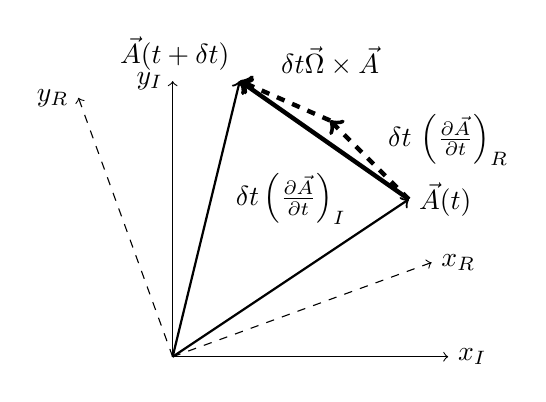
\begin{tikzpicture}
            \draw[->] (0,0) -- (3.5,0) node[anchor=west] {$x_I$};
            \draw[->] (0,0) -- (0,3.5) node[anchor=east] {$y_I$};
            \draw[thick,->] (0,0) -- (3,2) node[anchor=west] {$\vec{A}(t)$};
            %\draw[dotted,->] (0,0) -- (2,3) node[anchor=south] {};
            \draw[thick,->] (0,0) -- (0.853,3.503) node[anchor=south east] {$\vec{A}(t+\delta t)$};
            \draw[ultra thick,->,dashed] (3,2) -- (2,3) {};
            \node[] at (3.5,2.75) {$\delta t \, \left( \frac{\partial \vec{A}}{\partial t} \right)_R$};
            \draw[ultra thick,->,dashed] (2,3) -- (0.853,3.503) {};
            \node[] at (2,3.75) {$\delta t \vec{\Omega}\times\vec{A}$};
            \draw[->,dashed] (0,0) -- (3.289,1.197) node[anchor=west] {$x_R$};
            \draw[->,dashed] (0,0) -- (-1.197,3.289) node[anchor=east] {$y_R$};
            \draw[ultra thick,->] (3,2) -- (0.853,3.503);
            \node[] at (1.5,2) {$\delta t \left( \frac{\partial \vec{A}}{\partial t} \right)_I$};
        \end{tikzpicture}
        \caption{Change in $\vec{A}$ in the Inertial Coordinate System}
        \label{Inertial}
    \end{subfigure}
    \caption{The change in $\vec{A}$ in a rotating (\ref{Rotating}) and inertial (\ref{Inertial}) coordinate system. As seen in \ref{Inertial}, the change in the inertial coordinate system $\delta t \left( \frac{\partial \vec{A}}{\partial t} \right)_I$ (thick arrow) is equal to sum of the change in the rotating coordinate system $\left( \delta t \left( \frac{\partial \vec{A}}{\partial t} \right)_R \right)$ \textit{and} the rotation of the rotating coordinate system $\left(\delta t\,\vec{\Omega}\times\vec{A} \right)$ (thick dashed arrows).}
    \label{Inertial to Rotating}
\end{figure}
\begin{align}
    \left(\frac{d\vec{A}}{dt}\right)_I=\left(\frac{d\vec{A}}{dt}\right)_R+\vec{\Omega}\times\vec{A}
    \label{Rotating Relation}
\end{align}

If we let $\vec{A}=\vec{r}$, where $\vec{r}$ is the position of our fluid parcel, we can apply Equation \ref{Rotating Relation} twice to obtain an expression for the acceleration of a fluid parcel in a rotating coordinate system.
\begin{align*}
    \vec{u}_I &= \left( \frac{d\vec{r}}{dt} \right)_I\\
    &= \left( \frac{d\vec{r}}{dt} \right)_R+\vec{\Omega}\times \vec{r}\\
    \vec{u}_I & = \vec{u}_R+\vec{\Omega}\times \vec{r}\\
    \therefore \vec{a}_I & =
    \left( \frac{d\vec{u}_I}{dt} \right)_I\\
    &= \left( \frac{d\vec{u}_I}{dt} \right)_R+\vec{\Omega}\times \vec{u}_I\\
    &= \left( \frac{d\vec{u}_R}{dt} \right)_R
    +\vec{\Omega}\times\left( \frac{d\vec{r}}{dt} \right)_R
    +\vec{\Omega}\times\left( 
        \vec{u}_R+\vec{\Omega}\times \vec{r}
     \right)\\
    &=\vec{a}_R+2\vec{\Omega}\times\vec{u}_R+\vec{\Omega}\times\vec{\Omega}\times\vec{r}
\end{align*}

Therefore the acceleration in the rotating frame of reference $\vec{a}$ is equal to the acceleration in a inertial coordinate system summed with two fictitious\href{https://xkcd.com/123/}{$^*$}  forces: the \textbf{centrifugal force} and the \textbf{coriolis force}.
\begin{align}
    \vec{a}_R=\vec{a}_I+\underbrace{2\vec{\Omega}\times\vec{u}_R}_\text{Coriolis}
    +\underbrace{\vec{\Omega}\times\vec{\Omega}\times\vec{r}}_\text{Centrifugal}
\end{align}

The \textbf{centrifugal force} is the force that pushes objects away from the axis of rotation. This is the force that makes your arms fling out if you spin. The \textbf{coriolis force} is the force that diverts moving objects which move away or towards the axis of rotation. 

We have thus transformed Equation \ref{Navier Stokes} into a rotating coordinate system:
\begin{align}
    \frac{D\vec{u}}{Dt}+2\vec{\Omega}\times\vec{u}+\frac{1}{\rho}\vec{\nabla}p+g\vec{k}=-\vec{\Omega}\times\vec{\Omega}\times\vec{r}+\nu\vec{\nabla}^2\vec{u}+\frac{\nu}{3}\vec{\nabla}(\vec{\nabla}\cdot\vec{u})+\vec{F}\label{Navier Stokes Rotating}
\end{align}

\subsection{Local Cartesian Coordinates}

We have just learnt how to deal with coordinate systems that vary with time. We will now skim over (since the details aren't that interesting) how to deal with coordinate systems that vary with space.

We wish to use a coordinate system that follows the surface of the Earth, with the basis vectors $\hat{x}$, $\hat{y}$, $\hat{z}$, pointing in the east, north, and upwards (away from the centre of the Earth) directions. In this coordinate system, we define the position and velocity coordiates $(x,y,z)$ and $(u,v,w)$ as indicating distance and velocity in the east, north, and upwards directions, respectively. We further define the latitude $\phi\in[-\frac{\pi}{2},\frac{\pi}{2}]$ ($\phi=0$ indicates the equator, $\phi=\pm\frac{\pi}{2}$ is the north/south pole) and the radial distance $r$ where $r=a+z$ where $a=$ the radius of the Earth (see Figure \ref{LocCartes}).
\begin{figure}[H]
    \centering
    \scalebox{1.4}{
    \begin{tikzpicture},
        \begin{scope}[3d view={125}{25.26}]
            \draw[->,opacity=0.7] (0,0,0) -- (1.5,0,0) node[anchor=north east] {$x'$};
            \draw[->,opacity=0.7] (0,0,0) -- (0,1.5,0) node[anchor=north] {$y'$};
            \draw[->,opacity=0.7] (0,0,0) -- (0,0,1.5) node[anchor=north west] {$z'$};
            \draw[-,dashed] plot[domain=0:400,samples=41,smooth]({1.5*sin(\x)},{1.5*cos(\x)},{0});
            \draw[-,dashed] plot[domain=0:400,samples=41,smooth]({1.5*cos(0)*sin(\x)},{1.5*sin(0)*sin(\x)},{1.5*cos(\x)});
            \draw[-,dashed] plot[domain=0:360,samples=41,smooth]({1.0607*sin(\x)},{1.0607*cos(\x)},{1.0607});
            \coordinate (A) at (1.0607,0,1.0607);
            \draw[-] (0,0,0) -- (A);
            \draw[->,thick,mymagenta] (A) -- (0.7071,0,1.414);
            \draw[->,thick,mymagenta] (A) -- (1.0607,0.5,1.0607);
            \draw[->,thick,mymagenta] (A) -- (1.414,0,1.414);
            %\filldraw[fill=myorange,opacity=0.5] (1,0,0) .. controls +(0,0,0.8) and +(0.5,0.2,0) .. (0.7071,0,0.7071) -- (0,0,0);
            \filldraw[fill=myorange,opacity=0.5] (1,0,0) .. controls +(0,0,0.5) and +(0.1,0,-0.1) .. (0.7071,0,0.7071) -- (0,0,0);
        \end{scope}
        \begin{scope}
            \draw[-,dashed] plot[domain=0:400,samples=41,smooth]({1.5*sin(\x)},{1.5*cos(\x)});
            \node at (-0.5,1.2) {$y$};
            \node at (-0.2,0.8) {$x$};
            \node at (-0.8,0.95) {$z$};
            \node at (-0.35,0.04) {$\phi$};
        \end{scope}
    \end{tikzpicture}}
    \caption{Local Carteisan Coordinates. $(x',y',z')$ indicate our global cartesian coordinate system, while $(x,y,z)$ indicate our local cartesian coordinate system in magenta arrows.}
    \label{LocCartes}
\end{figure}
Churning through the algebra, we get:
\begin{align*}
    \frac{Du}{Dt}-\left( 2\Omega+\frac{u}{r\cos\phi} \right)\left( v\sin\phi-w\cos\phi \right)+\frac{1}{\rho}\frac{\partial p}{\partial x}
    =F_x\\
    \frac{Dv}{Dt}+\frac{wv}{r}+\left( 2\Omega+\frac{u}{r\cos\phi} \right)u\sin\phi+\frac{1}{\rho}\frac{\partial p}{\partial y}=F_y\\
    \frac{Dw}{Dt}-\frac{u^2+v^2}{r}-2\Omega u \cos\phi+\frac{1}{\rho}\frac{\partial p}{\partial z}+g=F_z
\end{align*}
where we have lumped together all the terms on the right-hand-side of \ref{Navier Stokes Rotating} into the $F_x, F_y, F_z$. Many of the extra terms $\left( \text{e.g., the } \frac{wv}{r} \text{ term}\right)$, are due to the fact that we have adopted a local cartesian system, in which the coordinate system changes as we move over the Earth. 

\subsection{Incompressibility}

This is in preparation for the next simplification we make: we assume that the fluid we are dealing with is \textbf{incompressible}\footnote{
    This should seem, to you, a highly dubious assumption. First, we know that sound waves are possible (after all we can hear, both on land and in water), but sound waves are impossible in an incompressible fluid. Second, we know that the atmosphere is approximately an ideal gas, which can have its density changed if warmed or cooled.
}. This implies that density is \textbf{Materially Conserved} following a fluid parcel. Therefore, for density $\rho$:
\begin{align}
    \frac{D\rho}{Dt}=0\nonumber\\
    \therefore \boxed{\vec{\nabla}\cdot \vec{u}=0}\label{Incompressible}
\end{align}
where we have obtained \ref{Incompressible} by substituting Mass Conservation (\ref{Mass Conservation}).

\subsection{Scale Analysis}

Finally, we make a few phenomenological simplifications. We do this here for simplicity, but our results are not general or particularily robust: these terms are essential in climate/weather models.
We do this here by performing a \textbf{scale analysis}: we estimate the size of quantities by their typical values (found empirically), then ignore terms that are much smaller than the other terms. We never neglect the pressure gradient term. \newline

\noindent
\begin{tabular}{|p{5.8cm}|p{1.4cm}|p{4cm}|p{4cm}|}
\hline
    Scale & Symbol & Terms Approximated & Typical Magnitude \\
\hline
\hline
Horizontal Scale & $L$ & $\frac{\partial}{\partial x}\sim\frac{1}{L}$, $\frac{\partial}{\partial y}\sim\frac{1}{L}$& \qty{e6}{\metre}\\
\hline
Vertical Scale & $H$ & $\frac{\partial}{\partial z}\sim\frac{1}{H}$& \qty{e4}{\metre}\\
\hline
Horizontal Velocity & $U$ & $u\sim U$, $v\sim U$& \qty{10}{\metre\per\second}\\
\hline
Vertical Velocity & $W$ & $w\sim W$& \qty{e-2}{\metre\per\second}\\
\hline
Time Scale & $T$ & $\frac{\partial}{\partial t}\sim\frac{1}{T}$& \qty{e5}{\second}\\
\hline
Density & $\rho$ & $\rho\sim\rho$& \qty{1}{\kilogram\per\second}\\
\hline
Earth's Radius & $a$ & $r\sim a$& \qty{6.4e6}{\metre}\\
\hline
Rotation Rate & $\Omega$ & $\Omega\sim\Omega$ & \qty{e-4}{\per\second}\\
\hline
Acceleration of Gravity & $g$ & $g\sim g$ & \qty{10}{\metre\per\second\squared}\\
\hline
\end{tabular}\newline

I do not write out all the details here, as they would easily take multiple pages. If you are curious about the details, refer to the mini-scale analysis I do in deriving \ref{Hydrostatic GFD}. A more rigorous method would be non-dimensionalisation, but this is overkill for our purposes. Again, if you are curious about the details, refer to the mini-non-dimensionalisation I do in deriving the \hyperref[Rossby Number]{Rossby Number}. 

Suffice it to say that we eliminate many terms through this scale analysis. This includes any terms that feature the viscosity $\nu$, the centrifugal force, and many terms arising from our local cartesian coordinate system. 

After eliminating small terms, we get our final simplified set of equations. 

\section{The Simplified Equations of Motion}

\begin{fact}{The Simplified Equations of Motion for GFD}{Eqns for GFD Box}\label{Eqns for GFD Box}
    We define the horizontal gradient operator taken at constant $z$ as $\vec{\nabla}_h=\left( \frac{\partial}{\partial x},\frac{\partial}{\partial x},0 \right)^T$, the horizontal velocity as $\vec{u}_h=\left( u,v,0 \right)^T$, the horizontal forces as $\vec{F}_h$, and the \textbf{coriolis parameter} as $f=2\Omega\sin\phi$ where $\phi=$ the latitude.

    The simplified equations of motion we will be using are as follows: 
    \begin{multicols}{2}
        \textbf{Horizontal Momentum Balance:}
        \begin{gather}
            \label{Horizontal Approximate}
            \BOX{\frac{D\vec{u}_h}{Dt}+f\vec{k}\times\vec{u}_h+\frac{1}{\rho}\vec{\nabla}_hp=\vec{F}_h}
        \end{gather}
        \textbf{Vertical Momentum Balance:}
        \begin{gather}
            \label{Vertical Approximate}
            \BOX{\frac{Dw}{Dt}+\frac{1}{\rho}\frac{\partial p }{\partial z}+g=F_z}
        \end{gather}
        \textbf{Mass Conservation:}
        \begin{gather}
            \label{Mass Material Conservation}
            \BOX{\frac{D\rho}{Dt}=0}
        \end{gather}
        \textbf{Incompressibility:}
        \begin{gather}
            \label{Incompressibility}
        \BOX{\vec{\nabla}\cdot\vec{u}=0}
        \end{gather}
    \end{multicols}
\end{fact}

Physically, the \textbf{coriolis parameter} $f=2\Omega \sin \phi$ is the planetary vorticity: it is the vorticity that a fluid parcel at rest (relative to the surface of the Earth) has in the $z$-direction.

We will mostly be dealing with the horizontal momentum equation \ref{Horizontal Approximate}, so it is worth detailing the meanings of each terms. The first term, $\frac{D\vec{u}_h}{Dt}$ is the material derivative of $\vec{u}_h$. It represents the acceleration of $\vec{u}_h$ and the advection of $\vec{u}_h$. The $f\vec{k}\times\vec{u}_h$ term is the acceleration due to coriolis. The $\frac{1}{\rho}\vec{\nabla}_h p$ is the force due to the horizontal pressure gradient. Finally, the $\vec{F}_h$ term is external forces, e.g., friction, wind-forcing, etc.

\begin{align*}
    \underbrace{\frac{D\vec{u}_h}{Dt}}_\text{acceleration and advection}+
    \overbrace{f\vec{k}\times\vec{u}_h}^\text{coriolis}+
    \underbrace{\frac{1}{\rho}\vec{\nabla}_hp}_\text{horizontal pressure gradients}=\overbrace{\vec{F}_h}^\text{other forces}
\end{align*}

\chapter{The Fundamental Diagnostic Relations}\label{Dia Relations}

\section{Hydrostatic Balance (Approximate Vertical Momentum Balance)}\label{App Vert Bal}

We now make further approximations to extract physical intuition. Consider \ref{Vertical Approximate}, and again perform a scale analysis and assume that $F_z\approx 0$.
\begin{align*}
    &&\frac{Dw}{Dt} &+
    & \frac{1}{\rho}\frac{\partial p}{\partial z}+
    &g=0
    \\
    &\underbrace{\frac{\partial w}{\partial t}}_{\frac{W}{T}}+ 
    &\underbrace{u\frac{\partial w}{\partial x} 
    + v\frac{\partial w}{\partial y}}_{U\frac{W}{L}}+ 
    &\underbrace{w\frac{\partial w}{\partial z}}_{W\frac{W}{H}}+ 
    &\frac{1}{\rho}\frac{\partial p}{\partial z}+
    &g=0
    \\
    &\sim\frac{W}{T}+
    &\sim U\frac{W}{L}+
    &\sim\frac{W^2}{H}+ 
    &\frac{1}{\rho}\frac{\partial p}{\partial z}+
    &g=0
    \\
    \therefore
    &\frac{\text{\qty{e-2}{\metre\per\second}}}{\text{\qty{e5}{\second}}}+ 
    &\text{\qty{10}{\metre\per\second}}\frac{\text{\qty{e-2}{\metre\per\second}}}{\text{\qty{e6}{\metre}}}+ 
    &\frac{\left( \text{\qty{e-2}{\metre\per\second}} \right)^2}{\text{\qty{e4}{\metre}}}+ 
    &\frac{1}{\rho}\frac{\partial p}{\partial z}+
    &\text{\qty{10}{\metre\per\second\squared}}=0
    \\
    &\text{\qty{e-7}{\metre\per\second\squared}}+
    &\text{\qty{e-7}{\metre\per\second\squared}}+
    &\text{\qty{e-8}{\metre\per\second\squared}}+
    &\frac{1}{\rho}\frac{\partial p}{\partial z}+
    &\text{\qty{10}{\metre\per\second\squared}}=0
    \\
    &\bcancel{\text{\qty{e-7}{\metre\per\second\squared}}}+
    &\bcancel{\text{\qty{e-7}{\metre\per\second\squared}}}+
    &\bcancel{\text{\qty{e-8}{\metre\per\second\squared}}}+
    &\frac{1}{\rho}\frac{\partial p}{\partial z}+
    &\text{\qty{10}{\metre\per\second\squared}}=0
\end{align*}

As seen then, many of the acceleration terms (the terms in the $\frac{Dw}{Dt}$) are 8 orders of magnitutde smaller than gravity! As such, the only term that can balance the gravity term is the pressure gradient. We thus neglect all other terms and derive again:

\begin{fact}{Hydrostatic Balance}{Hydrostatic GFD Box}\label{Hydrostatic GFD Box}
Hydrostatic Balance governs the vertical pressure variation in a fluid if we assume that vertical acceleration (and advection) is small.
    \begin{equation}\label{Hydrostatic GFD}
    \BOX{
        \frac{\partial p}{\partial z}=-\rho g
    }
    \end{equation}
Pressure decreases with height in order to balance the force of gravity.
\end{fact}

Physically, hydrostatic balance is a force/momentum balance in the vertical direction, where the force of gravity is balanced by the vertical pressure gradient. Notice now the difference between the Hydrostatic Balance I have written here (\ref{Hydrostatic GFD}) and the Hydrostatic Balance I have written in the \hyperref[Thermodynamics]{Thermodynamics} Section (\ref{Hydrostatic Balance}): I have written it here with a partial derivative. Strictly, it should have been a partial derivative before too, but I write it here to note that we are now considering horizontal variations as well as vertical variations.

For an ideal gas, one can substitute for $\rho$ using \ref{Ideal Gas}:
\begin{align}\label{Hydrostatic Ideal Gas}
    \boxed{\frac{\partial \ln p}{\partial z}=-\frac{g}{RT}}
\end{align}

\section{Geostrophic Balance (Approximate Horizontal Momentum Balance)}\label{App Horiz Bal}

\subsection{Rossby Number and Non-Dimensionalisation}

Let us now consider the horizontal momentum equation \ref{Horizontal Approximate} and let $\vec{F}_h\approx 0$ for now. We nondimensionalise the equations by defining dimensionless hatted variables and choosing characteristic scales such that the dimensionless hatted variables are of order 1:
\begin{align*}
    t=[t]\hat{t}\text{   ;   }
    \vec{r}=L\vec{\hat{r}}\text{   ;   }
    \vec{u}_h=[u_h]\vec{\hat{u}}_h\text{   ;   }
    p=[p]\hat{p}
\end{align*}

So, for example, $[t]= $ the timescale with dimensions of time and $L= $ the lengthscale with dimesions of length, while $\hat{t}$ and $\vec{hat{r}}$is the dimensionless time/position variables. We \textit{must} pick these scales $[t]$, $L$, $[u_h]$, $[p]$ \textit{such that} the hatted variables ($\hat{t}$,$\vec{\hat{r}}$, $\vec{\hat{u}}_h$, $\hat{p}$) are of order one, so we're constrained by the system under consideration.\footnote{
    In fact we've already made an implicit assumption that the system is roughly isotropic, which means that we can choose $[v]=[u]=[u_h]$ and $[x]=[y]=L$.  
} We now substitute these variables into \ref{Horizontal Approximate}:
\begin{align*}
    \frac{[u_h]}{[t]}\frac{\partial\vec{\hat{u}}_h}{\partial t}+\frac{[u_h]^2}{L}\left( \vec{\hat{u}}_h\cdot\vec{\hat{\nabla}} \right)\vec{\hat{u}}_h+[u_h]f\vec{k}\times\vec{\hat{u}}_h+[p]\frac{1}{\rho}\vec{\nabla}_h\hat{p}=0
\end{align*}
where $\vec{\hat{\nabla}}=(\partial/\partial \hat{x},\partial/\partial \hat{y})^T$ is the non-dimesional nabla operator. Dividing by $f[u_h]$, we get:
\begin{align*}
    \underbrace{\boxed{\frac{1}{f[t]}}}_{\equiv St}\frac{\partial\vec{\hat{u}}_h}{\partial t}+\underbrace{\boxed{\frac{[u_h]}{fL}}}_{\equiv Ro}\left( \vec{\hat{u}}_h\cdot\vec{\hat{\nabla}} \right)\vec{\hat{u}}_h+\vec{k}\times\vec{\hat{u}}_h+\underbrace{\boxed{\frac{[p]}{\rho f [u_h]}}}_{\equiv P}\vec{\nabla}_h\hat{p}=0
\end{align*}

We thus see three non-dimesional coefficients appear in front of each of the terms in each equation: $St$, $Ro$, and $P$.\footnote{
    While $St$ and $Ro$ are standard nomenclature for these non-dimesional quantities, $P$ is not.
} These non-dimesional coefficients compare the relative size and therefore importance each term in the Horizontal Momentum equation. You might expect there to be four non-dimesional coefficients because there were four scales we could choose, but there are only three because this fourth non-dimensional coefficient is set by the Horizontal Momentum equation itself: all the terms on the left hand side \textit{must} sum to $0$.

Now, written just in terms of the non-dimensional coefficients, we write the (isotropic) non-dimensional horizontal momentum equation:
\begin{align}
    \label{Horizontal Approximate nondim}
    \underbrace{St\,\frac{\partial\vec{\hat{u}}_h}{\partial t}}_{O(St)}+
    \underbrace{Ro\,\left( \vec{\hat{u}}_h\cdot\vec{\hat{\nabla}} \right)\vec{\hat{u}}_h}_{O(Ro)}+
    \underbrace{\vec{k}\times\vec{\hat{u}}_h}_{O(1)}+
    \underbrace{P\,\vec{\nabla}_h\hat{p}}_{O(P)}=0
\end{align}

Note that because we have nondimensionalised such that each variable is of order one, the $\vec{k}\times\vec{\hat{u}}_h$ is always of order one, while the other terms are of order $St$, $Ro$, and $P$, respectively.

The physical interpretation of each coefficient is as follows: $St$ represents the ratio of the intrinsic timescale of the system $[t]$ (set by dynamics of the particular problem under consideration) and the timescale of the rotation of the planet $1/f$. This intrinsic timescale could be set, for example, by the stratification (for example the Brunt Vasalla frequency you encountered in Clouds PUT REFERENCE HERE $[t]=1/N$). Other times, if there is no intrinsic timescale, the timescale is often set by the advection $[t]=L/[u_h]$. If this timescale is much shorter than the rotation timescale (i.e., if $[t]\ll 1/f$) then $St\gg 1$, so the left-hand most term is much larger than the rotation $\vec{k}\times\vec{\hat{u}}_h$ term. Physically, this means that the local rate of change `doesn't see' the fact that the planet is rotating. This is because everything happens so quickly that the planet hasn't rotated much to affect events. This is what happens on human scales: if I throw a ball at you then this takes much less time than $1/f\sim$ 1 day, so we don't notice the Earth rotating.

For simplicity, we simply assume at this point that the following obtains: that the timescale is set by advection or something slower than advection such that $[t]\geq L/[u_h]$ (i.e., we are never interested in stuff happening on very time-scales shorter than the advective timescale). As such, we can approximate $St\leq Ro$ so that we get:
\begin{align*}
    Ro\,\left( \frac{\partial\vec{\hat{u}}_h}{\partial t}+\left( \vec{\hat{u}}_h\cdot\vec{\hat{\nabla}} \right)\vec{\hat{u}}_h\right)+\vec{k}\times\vec{\hat{u}}_h +P\,\vec{\nabla}_h\hat{p}=0
\end{align*}

We can now explain the \textbf{Rossby Number} $Ro$ very easily. $Ro$ compares the effect of advection/acceleration to rotation: if $Ro \ll 1$ (the \textbf{Rossby Number} is small), then rotation is important and dominates dynamics. If $Ro \gg 1$ (the \textbf{Rossby Number} is large), then the flow evolves in such a way where coriolis is negligible.

\begin{fact}{Rossby Number}{Rossby box}\label{Rossby Box}
    We define the dimensionless \textbf{Rossby Number} $Ro$, which encodes the relative importance of (planetary) rotation and advection/acceleration terms, as follows:
    \begin{gather}
        \label{Rossby Number}
        \BOX{
            Ro=\frac{U}{fL}
        }
    \end{gather}
    where $U=$ the horizontal velocity scale, $f=$ the coriolis parameter, and $L=$ the horizontal length scale.
    
    If $Ro\ll 1$, then the rotation of the planet is important, and the flow should be approximately \textbf{Geostrophic}. If $Ro\gg 1$, then acceleration/advection is important.
\end{fact}

Note that I have not specified $P$. This is because we expect the pressure scale $P$ to be set by the dynamics governed by the \hyperref[Horizontal Approximate]{Horizontal Momentum Equation}. If $Ro\ll 1$, then we expect $P$ to be of order $1$ in order to balance the coriolis $\vec{k}\times\vec{\hat{u}}_h$ term. If $Ro\gg 1$, then we expect $P$ to be of order $Ro$ in order to balance the advection/acceleration $D\vec{\hat{u}}_h/Dt$ term. 

We can also write the Rossby Number in terms of a ratio between the planetary vorticity and relative vorticity. The planetary vorticity $\omega_{planetary}$ is the angular velocity of a fluid parcel due to the rotation of the Earth, and scales as $f$. The relative vorticity is the vorticity of our fluid parcel in our coordinate system which is rotating with the Earth, and scales as $\omega_{relative}\sim[\vec{\omega}]_z=[\vec{\nabla}\times\vec{u}_h]_z\sim U/L$. Therefore:
\begin{align}
    Ro &= \frac{\omega_{relative}}{\omega_{planetary}}\\
    &\sim\frac{U/L}{f}
\end{align}

The actual size of $Ro$ depends on the kind of system we are considering: i.e., what are the length-scales and velocity-scales of the system. But it also, crucially, depends on the coriolis parameter $f=2\Omega\sin\phi$. $f=0$ at or near the equator, and so it is unlikely that $Ro$ will ever be small near the equator. However, this does not imply that rotation is unimportant near the equator, but it does imply that the flow is probably not geostrophic near the equator.

Much of the theory of GFD that we will discuss will require the system to be geostrophic, or approximately geostrophic, which means that much of what we apply will only be very accurate in the mid-/high-latitudes (coincidentally where we are!). It is worth bearing this in mind.

\subsection{Geostrophic Balance}

If $Ro\ll 1$ and all other forces are negligible, then rotation dominates dynamics. We can therefore neglect external forces (set $\vec{F}_h\approx0$) and acceleration and advection (set $D\vec{u}_h/Dt\approx0$) in Equation \ref{Horizontal Approximate nondim} (the horizontal momentum equation). Because the equation must equal $0$, we are forced to conclude that $P$ is of order one, so Equation \ref{Horizontal Approximate nondim} and therefore Equation \ref{Horizontal Approximate} must be a balance between the horizontal pressure gradient force and the coriolis force.\footnote{
    You might be suspicious from what I've said. After all, $Ro$ depends on velocity-scale $U$ and length-scale $L$, which we expect should be set by the dynamics and governed by the underlying equations of motion!

    In other words, \textit{if} $Ro\ll 1$, then we expect the system to be in geostrophic balance, but why is $Ro\ll 1$ in the first place, and why would our atmosphere/ocean system tend towards a state such that $Ro\ll 1$ holds?

    The answer lies in the phenomenon of \textbf{geostrophic adjustment}, which you can read about in Vallis' textbook on GFD \cite{Vallis}. The gist is this: anomalies and instabilities on a rotating planet cannot simply propagate away (e.g., via gravity flattening the surface of a fluid, for example) from the source to make the fluid more homogenous. It cannot because the fluid is on a rotating planet, and so must preserve some form of angular momentum.

    As such, after anomalies begin propagating away, there will come a point (where it reaches the anomaly reaches the \hyperref[SW Def Radius Box]{Rossby Deformation Scale}) where it is deflected by the coriolis force, and the system evolves \textit{towards} geostrophic balance.

    More details, again, can be found in Vallis' book.
} 

\begin{fact}{Geostrophic Balance}{Geostrophic Box}\label{Geostrophic Box}
    A flow is geostrophic if the dominant terms in the horizontal momentum balance equation (Equation \ref{Horizontal Approximate}) are the coriolis force and the pressure gradient force. As such, these terms must balance as follows:
    \begin{align}
        \label{Geo Bal}
        \BOX{f\vec{k}\times\vec{u}_h=-\frac{1}{\rho}\vec{\nabla}_hp}
    \end{align}
    This results in a velocity field determined by the pressure gradient as follows (Exercise: Show that Equation \ref{Geostrophic Balance} satisfies Equation \ref{Geo Bal} for any arbitrary pressure field $p$):
    \begin{align}\label{Geostrophic Balance}
        \boxed{\vec{u}_h=\frac{1}{\rho f}\vec{k}\times\vec{\nabla}_hp}
    \end{align}
\end{fact}

Written out, each component of $\vec{u}_h=(u,v)^T$ is as follows:

\begin{minipage}{0.45\linewidth}
    \begin{align*}
        \BOX{u = -\frac{1}{\rho f}\frac{\partial p}{\partial y}}
    \end{align*}
\end{minipage}
\hfill
\begin{minipage}{0.45\linewidth}
    \begin{align*}
        \BOX{v = \frac{1}{\rho f}\frac{\partial p}{\partial x}}
    \end{align*}
\end{minipage}

Recall that the horizontal gradient of pressure $\vec{\nabla}_h p$ points in the direction of increasing $p$. Equation \ref{Geo Bal} shows that the coriolis force, which pushes a fluid at right angles to its velocity, balances the pressure gradient force, which pushes a fluid from areas of high pressure to areas of low pressure.

We can use Equation \ref{Ideal Gas} to show that, for an ideal gas, geostrophic balance may be written as follows:
\begin{align}
    \label{Geostrophic Ideal Gas}
    \vec{u}_h=\frac{RT}{ f}\vec{k}\times\vec{\nabla}_h\ln p
\end{align}

\subsection{Cyclones and Anti-Cyclones}\label{Cyclones}

The horizontal velocity field is thus set by the horizontal pressure field in Equation \ref{Geostrophic Balance}. 

Recall from our \hyperref[VC Interp]{Vector Calculus Interpretation Box} that the contours of constant $p$ are always perpendicular to the gradient $\vec{\nabla}_h p$ of the pressure field $p$, and point from areas of low pressure to areas of high pressure. Recall further that a cross product of two vectors $\vec{a}\times\vec{b}$ is always perpendicular to both $\vec{a}$ and $\vec{b}$.\footnote{
    The way I like to remember how this works is the right-hand rule. Make a cartesian coordinate system with your right hand: first make a thumbs up with your right hand, then point your index finger away from you, then point your middle fingle to your left.

    Now consider $\vec{a}\times\vec{b}=\vec{c}$. If you align $\vec{a}$ with your thumb, then align $\vec{b}$ with your index finger, then $\vec{c}$ will be pointing in the direction of your middle finger!

    Further note: (I think?) this is why we call certain cartesian coordinate systems a right handed coordinate system, because $\hat{x}\times\hat{y}=\hat{z}$, where $\hat{x}$, $\hat{y}$, $\hat{z}$ are the unit vectors pointing in the $x$, $y$, and $z$ directions.
}

Therefore, if the flow is geostrophic, then $\vec{u}_h$ flows parallel \textbf{isobars} (an isobar is defined as a contour of constant $p$). It is not difficult to verify this by showing that $\vec{u}_h\cdot\vec{\nabla}_h p=0$.

If you consider blobs of higher or lower pressure (which I will draw with circles for simplicity), you will see that the horizontal velocity flows either clockwise or anticlockwise around the areas of high or low pressure. Whether it is clockwise or anticlockwise will depend if we are in the northern hemisphere (so that $f=2\Omega\sin\phi>0$ obtains) or in the southern hemisphere (so that $f=2\Omega\sin\phi<0$ obtains).

\begin{figure}[H]
    \centering
    \begin{subfigure}{0.45\linewidth}
        \centering
        \begin{tikzpicture}
            \draw[fill=none](0,0) circle (1.5);
            \draw[fill=none](0,0) circle (3);
            \draw[->,thick,mydarkblue] (2.121,2.121) arc[start angle=45, end angle=225, radius=3cm];
            \draw[->,ultra thick,mymagenta,dotted] (2.121,2.121)--(1.131,1.131);
            \node[] at (0.831,1.831) {$-\frac{1}{\rho}\vec{\nabla}_h p$};
            \draw[->,ultra thick,myorange,densely dashed] (2.121,2.121)--(3.111,3.111);
            \node[] at (3.111,3.411) {$f\vec{k}\times\vec{u}_h$};
            \draw[->,ultra thick,mydarkblue] (2.121,2.121)--(1.131,3.111);
            \node[] at (1.131,3.411) {$\vec{u}_h$};
            \node[] at (0,0) {Low Pressure};
            \node[] at (0,-2.1) {Medium Pressure};
            \node[] at (0,-3.5) {High Pressure};
        \end{tikzpicture}
        \caption{Cyclone: a \textbf{Low} Pressure System. The fluid flows anti-clockwise around a cyclone in the northern hemisphere.}
    \end{subfigure}
    \hfill
    \begin{subfigure}{0.45\linewidth}
        \centering
        \begin{tikzpicture}
            \draw[fill=none](0,0) circle (1.5);
            \draw[fill=none](0,0) circle (3);
            \draw[->,thick,mydarkblue] (2.121,2.121) arc[start angle=45, end angle=-135, radius=3cm];
            \draw[->,ultra thick,myorange,densely dashed] (2.121,2.121)--(1.131,1.131);
            \node[] at (0.831,1.831) {$f\vec{k}\times\vec{u}_h$};
            \draw[->,ultra thick,mymagenta,dotted] (2.121,2.121)--(3.111,3.111);
            \node[] at (3.111,3.411) {$-\frac{1}{\rho}\vec{\nabla}_h p$};
            \draw[->,ultra thick,mydarkblue] (2.121,2.121)--(3.111,1.131);
            \node[] at (3.111,1.631) {$\vec{u}_h$};
            \node[] at (0,0) {High Pressure};
            \node[] at (0,-2.1) {Medium Pressure};
            \node[] at (0,-3.5) {Low Pressure};
        \end{tikzpicture}
        \caption{Anti-Cyclone: a \textbf{High} Pressure System. The fluid flows clockwise around an anti-cyclone in the northern hemisphere.}
    \end{subfigure}
    \caption{Cyclones and Anticyclones in the northern hemisphere ($f>0$). Isobars are drawn as solid black lines \textcolor{black}{\rule{0.25cm}{0.25cm}}., the pressure gradient force $\left( -\frac{1}{\rho}\vec{\nabla}_h p \right)$ as \textcolor{mymagenta}{thick dotted magenta arrows \rule{0.25cm}{0.25cm}}, the coriolis force $\left( f\vec{k}\times\vec{u}_h \right)$ as \textcolor{myorange}{thick dashed orange arrows \rule{0.25cm}{0.25cm}}, and the velocity $\left( \vec{u}_h \right)$ as \textcolor{mydarkblue}{thick filled dark blue arrows \rule{0.25cm}{0.25cm}}.}
\end{figure}

Now, of course, cyclones and anti-cyclones as I have described them here are theoretical approximations to \textit{actual} cyclones and anti-cyclones. One way in which actual cyclones/anti-cyclones differ is that they are subject to other forces, like friction with the ground or centrifugal forces. Another way in which actual cyclones/anti-cyclones differ is that they are three-dimensional, and we have not considered the vertical velocity in cyclones or anti-cyclones.

However, we do not yet have the vocabulary needed to fully describe such systems. We will have to postpone discussion regarding this for now.

Suffice it to say that cyclones and anti-cyclones are weather systems that propogate across the mid-/high-latitudes. They can be generated if there is energy to cause an area of high or low pressure, and they dissipate due to the effects of surface friction and potential vorticity (a concept we will cover later). Because of how cyclones and anti-cyclones interact with the ground and friction, cyclones result in areas of rising air, while anti-cyclones result in areas of sinking air. Thinking back to convection, this brings unsettled, cloudy, and rainy conditions in the former case.

\subsection{Gradient-Wind Balance}

We will now make a brief detour to analyse how the centrifugal force affects cyclones and anti-cyclones. 

I should be clear \textit{which} centrifugal force we are considering in this subsection. In this case, we are considering the the centrifugal force on the air parcel arising from the fact that the air parcel is moving in a circle \textit{around the centre of the cyclone or anti-cyclone}, and is therefore accelerating inwards towards the cyclone. This gives rise to a centrifugal force that pushes the air parcel away from the centre of the cyclone (in the frame of reference rotating with the cyclone/anti-cyclone).

We are \textit{not} considering the centrifugal force on the air parcel arising from the fact that air parcel is moving in a circle \textit{around the centre of the Earth} (due to the fact that the Earth is spinning), and is therefore accelerating inwards towards the centre of the Earth. This gives rise to a centrifugal force that pushes the air parcel away from the centre of the Earth (in the frame of reference rotating with the Earth but not the cyclone/anti-cyclone). 

Now that we've gotten this potential confusion out the way, consider an air parcel moving in circular motion around a centre of high or low pressure. We adopt a local polar coordinate system, with the coordinates $(r,\theta)$ where $x=r\cos\theta$ and $y=r\sin\theta$. We assume there are no forces in the $\theta$-direction and only consider forces in the $r$-direction.

In this direction, there are three forces on the air parcel. We already considered the first two: the pressure gradient force $\left( -\frac{1}{\rho}\vec{\nabla}_h p = -\frac{1}{\rho}\frac{\partial p}{\partial r} \hat{r} \right)$ and the coriolis force $\left( f\vec{k}\times \vec{u}_h = fu_h\hat{r}  \right)$ where $u_h=|\vec{u}_h|$ and $\hat{r}$ is the unit vector pointing in the $r$-direction. Since the air parcel is moving in circular motion, we know that it is subject to a centrifugal force away from the vortex with magnitude $\frac{u_h^2}{r}\hat{r}$.\footnote{Equivalently, we can say that the parcel must be accelerating inwards with an acceleration of $-\frac{u_h^2}{r}\hat{r}$}. For an cyclone and an anti-cyclone in the northern hemisphere, it will look as follows:

\begin{figure}[H]
    \centering
    \begin{subfigure}{0.45\linewidth}
        \centering
        \begin{tikzpicture}
            \draw[fill=none](0,0) circle (1.5);
            \draw[fill=none](0,0) circle (3);
            \draw[->,thick,mydarkblue] (2.121,2.121) arc[start angle=45, end angle=225, radius=3cm];
            \draw[->,ultra thick,mymagenta,dotted] (2.121,2.121)--(1.131,1.131);
            \node[] at (0.831,1.831) {$-\vec{\nabla}_h p$};
            \draw[->,ultra thick,myorange,densely dashed] (2.121,2.121)--(3.111,3.111);
            \node[] at (3.111,3.411) {$f\vec{k}\times\vec{u}_h+\frac{u_h^2}{r}$};
            \draw[->,ultra thick,mydarkblue] (2.121,2.121)--(1.131,3.111);
            \node[] at (1.131,3.411) {$\vec{u}_h$};
            \node[] at (0,0) {Low Pressure};
            \node[] at (0,-2.1) {Medium Pressure};
            \node[] at (0,-3.5) {High Pressure};
        \end{tikzpicture}
        \caption{Cyclone: a \textbf{Low} Pressure System. The fluid flows anti-clockwise around a cyclone in the northern hemisphere.}
    \end{subfigure}
    \hfill
    \begin{subfigure}{0.45\linewidth}
        \centering
        \begin{tikzpicture}
            \draw[fill=none](0,0) circle (1.5);
            \draw[fill=none](0,0) circle (3);
            \draw[->,thick,mydarkblue] (2.121,2.121) arc[start angle=45, end angle=-135, radius=3cm];
            \draw[->,ultra thick,myorange,densely dashed] (2.121,2.121)--(1.131,1.131);
            \node[] at (0.831,1.831) {$f\vec{k}\times\vec{u}_h$};
            \draw[->,ultra thick,mymagenta,dotted] (2.121,2.121)--(3.111,3.111);
            \node[] at (3.111,3.411) {$-\vec{\nabla}_h p+\frac{u_h^2}{r}$};
            \draw[->,ultra thick,mydarkblue] (2.121,2.121)--(3.111,1.131);
            \node[] at (3.111,1.631) {$\vec{u}_h$};
            \node[] at (0,0) {High Pressure};
            \node[] at (0,-2.1) {Medium Pressure};
            \node[] at (0,-3.5) {Low Pressure};
        \end{tikzpicture}
        \caption{Anti-Cyclone: a \textbf{High} Pressure System. The fluid flows clockwise around an anti-cyclone in the northern hemisphere.}
    \end{subfigure}
    \caption{Gradient Wind Balance with cyclones and anticyclones in the northern hemisphere ($f>0$). Isobars are drawn as solid black lines \textcolor{black}{\rule{0.25cm}{0.25cm}}., the pressure gradient force $\left( -\frac{1}{\rho}\vec{\nabla}_h p \right)$ as \textcolor{mymagenta}{thick dotted magenta arrows \rule{0.25cm}{0.25cm}}, the coriolis force $\left( f\vec{k}\times\vec{u}_h \right)$ as \textcolor{myorange}{thick dashed orange arrows \rule{0.25cm}{0.25cm}}, and the velocity $\left( \vec{u}_h \right)$ as \textcolor{mydarkblue}{thick filled dark blue arrows \rule{0.25cm}{0.25cm}}.}
\end{figure}

Notice how, for a cyclone, the centrifugal force points in the same direction as the coriolis force. For an anti-cyclone, the centrifugal force points in the opposite driection as the coriolis force (i.e., in the direction of the pressure gradient force).

Therefore, if the pressure gradient force is of a similar size for both a cyclone and anti-cyclone, we should expect the coriolis force to be \textit{smaller} in a cyclone than in an anticyclone. Since the corilis force scales as the wind speed $u_h$, we expect a cyclone to produce \textit{weaker} winds than an anti-cyclone for the same pressure gradients. Turning this on its head, if a cyclone and an anti-cyclone have similar wind-speeds, we expect the cyclone to have \textit{stronger} pressure gradients.

\section{Thermal Wind Balance}

Now that we have covered the fundamental diagnostic relations of \hyperref[Hydrostatic GFD Box]{Hydrostatic Balance} and \hyperref[Geostrophic Box]{Geostrophic Balance}, we now aim to put these two pieces of information together to find a relation between the horizontal velocity $\vec{u}_h$ and the temperature in an ideal gas atmosphere.

We begin with Equations \ref{Hydrostatic Ideal Gas} and \ref{Geostrophic Ideal Gas} expressing respectively hydrostatic and geostrophic balance for an ideal gas. We first take the partial derivative with respect to $z$ of Equation \ref{Geostrophic Ideal Gas}:
\begin{align*}
    \frac{\partial\vec{u}_h}{\partial z}&=\frac{\partial}{\partial z} \left( \frac{R}{f}\vec{k}\times \left( T\vec{\nabla}_h \ln p \right) \right)
    &
    \text{ ; }
    &
    \frac{\partial}{\partial z}\text{ of Eqn. \ref{Geostrophic Ideal Gas}}
    \\
    &=\frac{R}{f}\vec{k}\times\left( 
        \frac{\partial T}{\partial z}\vec{\nabla}_h \ln p
        +
        T\vec{\nabla}_h \frac{\partial \ln p}{\partial z}
     \right)
    &
    \text{ ; }
    &
    \text{Assume }\frac{\partial \bar{M}}{\partial z}=0\text{ and that partial derivatives commute}
    \\
    &=\frac{R}{f}\vec{k}\times\left( 
        \frac{\partial T}{\partial z}\vec{\nabla}_h \ln p
        -
        T\vec{\nabla}_h \frac{g}{RT}
    \right)
    &
    \text{ ; }
    &
    \text{Substitute Eqn. \ref{Hydrostatic Ideal Gas} for }\frac{\partial \ln p}{\partial z}
    \\
    &=\frac{R}{f}\vec{k}\times\left( 
        \frac{\partial T}{\partial z}\vec{\nabla}_h \ln p
        +
        \frac{g}{RT}
        \vec{\nabla}_h T
    \right)
    &
    \text{ ; }
    &
    \text{Apply chain rule}
    \\
    &=\frac{R}{f}\vec{k}\times\left( 
        \frac{\partial T}{\partial z}\frac{f}{RT} \vec{k}\times\vec{u}_h
        +
        \frac{g}{RT}
        \vec{\nabla}_h T
    \right)
    &
    \text{ ; }
    &
    \text{Substitute Eqn. \ref{Geo Bal} for }\vec{\nabla}_h\ln p
\end{align*}

Now we estimate each term in the final brackets in the final equation:
\begin{align*}
    \frac{\partial \vec{u}_h}{\partial z}=\frac{1}{fT}\vec{k}\times\biggl( 
        \underbrace{\overbrace{\frac{\partial T}{\partial z}}^{\sim\qty{1e-2}{\kelvin\per\meter}}
        \overbrace{f}^{\sim\qty{1e-5}{\per\second}}
        \vec{k}\times
        \overbrace{\vec{u}_h}^{\sim\qty{10}{\meter\per\second}}}_{\sim \qty{1e-6}{\kelvin\per\square\second}}
        +
        \underbrace{\overbrace{g}^{\sim\qty{10}{\meter\per\square\second}}
        \overbrace{\vec{\nabla}_h T}^{\sim\qty{1e-5}{\kelvin\per\meter}}}_{\sim\qty{1e-4}{\kelvin\per\square\second}}
    \biggr)
\end{align*}

So we see that even though horizontal temperature gradients $\vec{\nabla}_h T$ are typically $1000$ times weaker than vertical temperature gradients $\frac{\partial T}{\partial z}$ (recall that horizontal temperature gradients roughly follow the Lapse Rate in Equation \ref{Dry Adiabatic Lapse Rate}), it is the term that features the horizontal temperature gradient that ends up begin much larger than the term that features the vertical temperature gradient.

As such, we neglect\footnote{
    We do not actually have to neglect this term when we derive these equations in pressure coordinates!
} the term on the left in the equation, and derive the \textbf{Thermal Wind Equations}:
\begin{align}\label{Thermal Wind}
    \BOX{\frac{\partial\vec{u}_h}{\partial z}\approx\frac{g}{fT}\vec{k}\times\vec{\nabla}_hT}
\end{align}

Written out, each component of $\vec{u}_h=(u,v)^T$ is as follows:

\begin{minipage}{0.45\linewidth}
    \begin{align}
        \label{u Thermal}
        \BOX{\frac{\partial u}{\partial z} \approx-\frac{g}{f T}\frac{\partial T}{\partial y}}
    \end{align}
\end{minipage}
\hfill
\begin{minipage}{0.45\linewidth}
    \begin{align}
        \label{v Thermal}
        \BOX{\frac{\partial v}{\partial z} \approx \frac{g}{f T}\frac{\partial T}{\partial x}}
    \end{align}
\end{minipage}

The physical interpretation is as follows: if the system is approximately both \hyperref[Geostrophic Box]{Geostrophic} and \hyperref[Hydrostatic GFD Box]{Hydrostatic}, and obeys ideal gas law, then horizontal temperature gradients imply vertical velocity gradients (and vice versa).

Let us now consider the vertical component of the vorticity. Recall that the voriticity is defined as follows: $\vec{\omega}=\vec{\nabla}\times\vec{u}$. Therefore the vertical component is given by: $[\vec{\omega}]_z=\xi=\frac{\partial v}{\partial x}-\frac{\partial u}{\partial y}$. If we differentiate Equations \ref{u Thermal} and \ref{v Thermal} with respect to $y$ and $x$ (respectively), then subtract them we can find an equation governing $\xi$:
\begin{align}
    \frac{\partial}{\partial x}\left( \frac{\partial v}{\partial z} \right) - \frac{\partial}{\partial y}\left( \frac{\partial u}{\partial z} \right)
    \approx
    \frac{g}{fT}\left( 
        \frac{\partial^2 T}{\partial x^2}+\frac{\partial^2 T}{\partial y^2}
     \right)\nonumber
     \\
    \label{Thermal Wind Vorticity}
    \therefore
    \BOX{
        \frac{\partial}{\partial z}\left( \frac{\partial v}{\partial x}- \frac{\partial u}{\partial y} \right)=
        \frac{\partial \xi}{\partial z}
        \approx
        \frac{g}{fT}\vec{\nabla}_h^2 T
    }
\end{align}

Now in the \hyperref[VC Interp]{Vector Calculus Interpretation Box} we interpreted the meaning of the gradient of a scalar field, but we are yet to interpret the \textbf{divergence} of the \textbf{gradient} of a scalar field. In this case, we specifically considering $\vec{\nabla}_h^2 T$.

This encodes the \textit{curvature} of the temperature scalar field $T(\vec{r},t)$. You will find that, if the temperature is constant or if the temperature increases at a constant rate in some direction, that this will be $0$. However, if the temperature increases then decreases, or increases more and more, then this will be non-zero.

Therefore, Equation \ref{Thermal Wind Vorticity} essentially says that the vertical gradient of the vorticity $\xi$ is set by the curvature of the temperature field $T$. 

This might make more sense with a concrete example. Suppose that we have a blob of cold air, i.e., we have a temperature field $T(\vec{r})$ that is minimum at the centre of the blob and warmer around the blob. If we consider $\vec{\nabla}_h T(\vec{r})$ (which I remind you is a vector field which points from low $T$ to high $T$), we would expect the vector field to look like arrows pointing away from the cold centre. Therefore the divergence of this vector field $\vec{\nabla}_h^2 T$ will be \textbf{positive} at this cold blob.

If you wan't to think of this in terms of curvature, since the temperature decreases then increases again when you pass through this cold blob, this implies that the temperature field $T(\vec{r})$ must be curved.  

Using Equation \ref{Thermal Wind Vorticity} $\vec{\nabla}_h^2 T>0$ therefore implies that $\frac{\partial \xi}{\partial z}>0$ (in the northern hemisphere), therefore the vertical vorticity increases with height in this cold blob! Vice versa for a hot blob in the northern hemisphere: in a hot blob will have vorticity decreasing with height. 

\section{Pressure Coordinates}\label{Pressure Coords}
\subsection{Partial Derivative Identities}

To convert to pressure coordinates we must first introduce some identities from vector calculus involving partial derivatives. We will skip the proof, so you'll just have to take the following identities on trust:
\begin{align*}
    \left(\frac{\partial a}{\partial b}\right)_{c,d}=\left(\frac{\partial b}{\partial a}\right)_{c,d}^{-1}
\end{align*}
\begin{align*}
    \left(\frac{\partial a}{\partial b}\right)_c
    \left(\frac{\partial b}{\partial c}\right)_a
    \left(\frac{\partial c}{\partial a}\right)_b
    =-1
\end{align*}
where we have explicitly written which variables are held constant in the subscripts. We apply this to $p$ and $z$:
\begin{align}
    \label{P inverse}
    \left(\frac{\partial p}{\partial z}\right)_{x,y}=\left(\frac{\partial z}{\partial p}\right)_{x,y}^{-1}
\end{align}
\begin{align*}
    \left(\frac{\partial p}{\partial x}\right)_z
    \left(\frac{\partial x}{\partial z}\right)_p
    \left(\frac{\partial z}{\partial p}\right)_x
    =-1
\end{align*}
\begin{align*}
    \left(\frac{\partial p}{\partial y}\right)_z
    \left(\frac{\partial y}{\partial z}\right)_p
    \left(\frac{\partial z}{\partial p}\right)_y
    =-1
\end{align*}
where the last two equations become:
\begin{align}
    \label{P -1}
    \left(\vec{\nabla}_h p\right)_z=-\left(\vec{\nabla}_h z\right)_p\left(\frac{\partial p}{\partial z}\right)_{x,y}
\end{align}

We must be careful with which variables we are actually holding constant when transforming from height coordinates to pressure coordinates. Before this section, we have implicitly held $z$ constant when calculating horizontal derivatives like $\frac{\partial}{\partial x}$ or $\frac{\partial}{\partial x}$. In practice, you should memorise Equations \ref{P inverse} and \ref{P -1} if you wish to reproduce this in an exam.

We will now apply this to four equations: \hyperref[Hydrostatic GFD Box]{hydrostatic balance} (\ref{Hydrostatic GFD}), \hyperref[Geostrophic Box]{geostrophic balance} (\ref{Geostrophic Balance}), thermal wind balance (\ref{Thermal Wind}), and mass conservation (\ref{Mass Material Conservation}) to derive their equivalent form in pressure coordinates. 

\subsection{Hydrostatic Balance}

Starting first from the hydrostatic relation (Equation \ref{Hydrostatic GFD}), we derive the equivalent relation expressing hydrostatic balance but in pressure coordinates using Equation \ref{P inverse}:
\begin{align*}
    -\rho g &= \left( \frac{\partial p}{\partial z} \right)_{x,y}
    \\
    &=\left( \left( \frac{\partial z}{\partial p} \right)_{x,y} \right)^{-1}
\end{align*}
\begin{align}
    \label{Hydrostatic Pressure}
    \therefore \BOX{
        \left( \frac{\partial \Phi}{\partial p} \right)_{x,y}
        =-\frac{1}{\rho}
    }
\end{align}
where we have defined the \textbf{geopotential height} $\Phi$ as follows:
\begin{align}
    \BOX{\Phi =g\,z}
\end{align}
There is nothing special about \textbf{geopotential height}. You can literally just think of \textbf{geopotential height} $\Phi$ as the height variable $z$ multiplied by $g$.

If we assume that the atmosphere consists of an ideal gas, then the following relation is the analogue for Equation \ref{Hydrostatic Balance Ideal}:
\begin{align}
    \boxed{\frac{\partial \Phi}{\partial \ln p}=-RT}
    \label{Hydrostatic Pressure Ideal}
\end{align}

\subsection{Geostrophic Balance}

We now turn to geostrophic balance. Again, starting from Equation \ref{Geostrophic Balance} but this time applying Equaiton \ref{P -1}:
\begin{align*}
    \vec{u}_h &= \frac{1}{\rho f}\vec{k}\times\left(\vec{\nabla}p\right)_z
    \\
    &=\frac{1}{\rho f}\vec{k}\times\left( 
        -\left( \vec{\nabla}_h z \right)_p \left( \frac{\partial p}{\partial z} \right)_{x,y}
     \right)
    \\
    &=\frac{1}{\rho f}\vec{k}\times\left( 
        -\left( \vec{\nabla}_h z \right)_p (-\rho g)
    \right)
\end{align*}
\begin{align}
    \label{Geostrophic Pressure}
    \therefore \BOX{
        \vec{u}_h = \frac{1}{f}\vec{k}\times\left( \vec{\nabla}_h \Phi \right)_p
    }
\end{align}
where we have used \hyperref[Hydrostatic GFD Box]{hydrostatic balance} to substitute for $\frac{\partial p}{\partial z}$. Each component of $\vec{u}_h$ is as follows:

\begin{minipage}{.48\linewidth}
    \begin{align*}
        \BOX{
            u = -\frac{1}{f}\left( \frac{\partial \Phi}{\partial y} \right)_p
        }
    \end{align*}
\end{minipage}
\hfill
\begin{minipage}{.48\linewidth}
    \begin{align*}
        \BOX{
            v = \frac{1}{f}\left( \frac{\partial \Phi}{\partial x} \right)_p
        }
    \end{align*}
\end{minipage}

\subsection{Thermal Wind Balance}

Thermal Wind Balance is particularly elegant in pressure coordinates, as we do not need to make the awkward scale analysis approximation we did in deriving Equation \ref{Thermal Wind} in height coordinates. We still need to assume that the system is in hydrostatic and geostrophic balance, and that the system is an ideal gas. To derive thermal wind balance in pressure coordinates, we simply take the derivative of Equation \ref{Geostrophic Pressure} with respect to $\ln p$ (and make use of Equation \ref{Hydrostatic Pressure Ideal}):
\begin{align*}
    \left( \frac{\partial}{\partial \ln p} \right)_{x,y}\left( \vec{u}_h \right)
    &= \left( \frac{\partial}{\partial \ln p} \right)_{x,y}
    \left( \frac{1}{f}\vec{k}\times\left( \vec{\nabla}_h \Phi \right)_p \right)
    \\
    &= \frac{1}{f}\vec{k}\times\left( \vec{\nabla}_h \left( \frac{\partial \Phi}{\partial \ln p} \right)_{x,y} \right)_{p}
    \\
    &= \frac{1}{f}\vec{k}\times\left( \vec{\nabla}_h (-RT) \right)_{p}
\end{align*}
\begin{align}
    \therefore
    \BOX{
        \left( \frac{\partial \vec{u}_h}{\ln p} \right)_{x,y}
        =
        -\frac{R}{f}\vec{k}\times \left( \vec{\nabla}_h T \right)_p
    }
\end{align}
Again, each component of $\vec{u}_h$ is as follows:

\begin{minipage}{.48\linewidth}
    \begin{align*}
        \BOX{
            \left( \frac{\partial u}{\partial \ln p} \right)_{x,y}
            =\frac{R}{f}
            \left( \frac{\partial T}{\partial y} \right)_{p}
        }
    \end{align*}
\end{minipage}
\hfill
\begin{minipage}{.48\linewidth}
    \begin{align*}
        \BOX{
            \left( \frac{\partial v}{\partial \ln p} \right)_{x,y}
            =-\frac{R}{f}
            \left( \frac{\partial T}{\partial x} \right)_{p}
        }
    \end{align*}
\end{minipage}

\subsection{Mass Conservation}

A final implication of converting to pressure coordinates is that we now have a new `vertical velocity'. The old vertical velocity was defined as follows:
\begin{align*}
    w_z = \frac{D z}{Dt}
\end{align*}
However, in pressure coordinates, we now define `vertical velocity' as follows:
\begin{align*}
    w_p = \frac{D p}{Dt}
\end{align*}

Again, assuming that the system is hydrostatic allows us to approximate $w_p$ the following way\footnote{
    Recall that the hydrostatic relation assumes that vertical variations in $p$ are dominant, therefore we can approximate the material derivative of $p$ as just the vertical advection component.
}:
\begin{align*}
    w_p &= \biggl( \underbrace{\frac{\partial }{\partial t} + u\left( \frac{\partial}{\partial x} \right)_{z}+v\left( \frac{\partial}{\partial y} \right)_{z}}_{\text{small }\therefore \text{ neglect}}+\underbrace{w_z \frac{\partial}{\partial z}}_{\text{big}} \biggr)\, p
    \\
    &\approx w_z \left( \frac{\partial p}{\partial z} \right)_{x,y}
    \\
    & = -w_z\rho g
\end{align*}

Recall Equation \ref{Mass Conservation} \ref{Mass Material Conservation} which states the following (this applies for both incompressible and compressible fluids):
\begin{align*}
    \frac{D\rho}{Dt}+\rho\vec{\nabla}\cdot\vec{u}=0
\end{align*}

Writing this in pressure coordinates gives us:
\begin{align*}
    0&=\left( 
        \frac{\partial}{\partial t} 
        + \vec{u}_h \cdot \left( \vec{\nabla}_h \right)_z
        + w_z \frac{\partial}{\partial z}
    \right)\rho
    + \rho \left( 
        \left( \vec{\nabla}_h  \right)_z \cdot \vec{u}_h
        + \frac{\partial}{\partial z}w_z
    \right)
    \\
    &=\left( 
        \frac{\partial}{\partial t} 
        + \vec{u}_h \cdot \left( \vec{\nabla}_h \right)_z
        - \frac{w_p}{\rho g} \frac{\partial p}{\partial z}\frac{\partial}{\partial p}
    \right)\rho
    + \rho \left( 
        \left( \vec{\nabla}_h  \right)_z \cdot \vec{u}_h
        - \frac{\partial p}{\partial z} \frac{\partial}{\partial p} \frac{w_p}{\rho g}
    \right)
    \\
    &=\left( 
        \frac{\partial}{\partial t} 
        + \vec{u}_h \cdot \left( \vec{\nabla}_h \right)_z
        + w_p \frac{\partial}{\partial p}
    \right)\rho
    + \rho \left( 
        \left( \vec{\nabla}_h  \right)_z \cdot \vec{u}_h
        +\rho g \frac{\partial}{\partial p} \frac{w_p}{\rho g}
    \right)
\end{align*}


Recall Equation \ref{Mass Conservation} which states the following (for an incompressible fluid):
\begin{align*}
    \frac{D\rho}{Dt}=\left( \frac{\partial }{\partial t} + u\left( \frac{\partial}{\partial x} \right)_{z}+v\left( \frac{\partial}{\partial y} \right)_{z}+w_z \frac{\partial}{\partial z}\right)\rho = 0
\end{align*}





\chapter{The Shallow Water System: 2D System}\label{Shallow Water System}

\section{The Equations of Motion}

In the previous chapter, we considered diagnostic relations: \hyperref[Hydrostatic GFD Box]{Hydrostatic Balance} and \hyperref[Geostrophic Box]{Geostrophic Balance}. These are very useful and important relations, but notice that there are no time derivatives in \ref{Hydrostatic GFD} and \ref{Geostrophic Balance}. If there are no time-derivatives, the equations cannot reproduce non-steady state solutions and time-evolution. However, clearly, the atmosphere and ocean evolve and are not in a steady state, and we wish to understand this.

Our first tool to consider time-dependent changes is the shallow water system. We consider a system governed the following equations and looks like this:

\begin{fact}{The Shallow Water System}{shallow box}\label{shallow box}

    The Shallow Water System is a simple two-dimensional time-varying system governing the evolution of a thin layer of incompressible fluid subject only to the pressure gradient and coriolis force.

    The three state variables are the horizontal velocity $\vec{u}_h(x,y,t)=(u,v)^T$ and the layer thickness $h(x,y,t)$. Equivalently, we can express the state variables as the horizontal velocity $\vec{u}_h(x,y,t)=(u,v)^T$ and the layer height $\eta(x,y,t)$.

    \begin{minipage}{.5\linewidth}
    \begin{gather}
        \label{SW mom}
        \BOX{\frac{D_h\vec{u}_h}{Dt}+f\vec{k}\times\vec{u}_h+g\vec{\nabla}_h\eta=0}\\
        \label{SW mass}
        \BOX{\frac{\partial h}{\partial t}+\vec{\nabla}_h\cdot(h\vec{u}_h)=0}\\
        \label{SW height}
        \BOX{h=\eta-b}
    \end{gather}
    where $\frac{D_h}{Dt}=\frac{\partial}{\partial t}+u\frac{\partial}{\partial x}+v\frac{\partial}{\partial y}=$ the horizontal material derivative, $\eta(x,y,t)=$ the height of the surface interface, and $b(x,y)=$ the bottom interface (which is given).
    \end{minipage}
    \hfill
    \begin{minipage}{.48\linewidth}
    \begin{figure}[H]
        \centering
        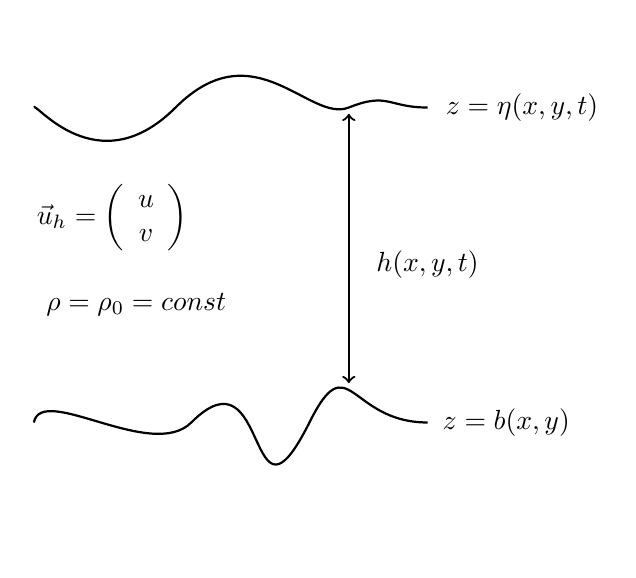
\begin{tikzpicture}
            \draw[thick] (0,0) .. controls +(0.1,0.5) and +(-0.5,-0.5) .. (2,0) .. controls +(1,1) and +(-0.8,-1.6) .. (3.5,0) .. controls +(0.5,1) and +(-1,0) .. (5,0);
            \node[] at (6,0) {$z=b(x,y)$};
            \draw[thick] (0,4) .. controls +(0,0.1) and +(-1,-1) .. (1.8,4) .. controls +(1,1) and +(-0.5,-0.2) .. (4,4) .. controls +(0.5,0.2) and +(-0.5,0) .. (5,4);
            \node[] at (6.2,4) {$z=\eta(x,y,t)$};
            \draw[thick,<->] (4,3.92) -- (4,0.5);
            \node[] at (5,2) {$h(x,y,t)$};
            \node[] at (1.3,1.5) {$\rho=\rho_0=const$};
            \node[] at (1,2.6) {$\vec{u}_h=\left( \begin{array}{c}u\\v\end{array} \right)$};
        \end{tikzpicture}
        \caption{The Shallow Water System}
    \end{figure}
    \end{minipage}
\end{fact}

We now aim to derive these equations from three primitive (approximate) equations: the horizontal momentum equation (\ref{Horizontal Approximate}), the vertical momentum equation (\ref{Vertical Approximate}), and mass conservation (\ref{Mass Conservation}). First, we neglect all vertical and horizontal forces $F_z$ and $\vec{F}_h$ (e.g. neglect friction) other than gravity and pressure gradient forces.

Second, we assume that the density is constant $\rho=\rho_0$ for all time and at all points. This immediately implies (from Equation \ref{Mass Conservation}) that the system must be incompressible, so we know that Equation \ref{Incompressibility} holds.

Third, we assume that the system is \textbf{shallow}: $H/L\ll 1$ where $H$ is the vertical lengthscale and $L$ is the horizontal lengthscale. If we non-dimensionalise \ref{Incompressibility}, we derive that the vertical velocity scale $W$ is much smaller than the horizontal velocity scale $U$: $W\ll U$:
\begin{align*}
    \vec{\nabla}\cdot\vec{u}=0\\
    \underbrace{\vec{\nabla}_h\cdot\vec{u}_h}_{U/L}+\underbrace{\frac{\partial w}{\partial z}}_{W/H}=0\\
    \therefore \frac{U}{L}\sim\frac{W}{H}\text{   }\therefore
    \frac{W}{U}\sim\frac{H}{L}\\
    \therefore \boxed{W \ll U}
\end{align*}

We take this as justification for our fourth assumption: that vertical acceleration and advection is small compared to gravity and pressure gradient forces. As such, the system is in approximately in \hyperref[Hydrostatic GFD]{Hydrostatic Balance} (we have simplified Equation \ref{Vertical Approximate} here). Importantly, though, we do \textit{not} assume that the vertical acceleration/advection is $0$ everywhere. We simply assume that they are much smaller than vertical pressure gradients and gravity.

This allows us to integrate the hydrostatic relation from some reference height $\eta$ (the height of the surface) and pressure $p_s$ (the pressure at the surface) to find that the following holds (refer to Equation \ref{Const Density Hydrostatic} to see the derivation).
\begin{align*}
    p(x,y,z,t)=\rho g(\eta(x,y,t)-z)+p_s(x,y,t)
\end{align*}

Fifth, we assume that the fluid above the layer of fluid under consideration has a much lower viscocity than the current layer or that it is much less dense than the other positions. This allows us to assume that $\vec{\nabla}_hp_s\ll \vec{\nabla}_h\eta$, and that therefore $\vec{\nabla}_h p \approx \rho_0 g \vec{\nabla}_h \eta$. As such, Equation \ref{Horizontal Approximate} becomes the following:
\begin{align*}
    \frac{D\vec{u}_h}{Dt}+f\vec{k}\times\vec{u}_h=g\vec{\nabla}_h\eta
\end{align*}

Notice that everything on the right hand side has no dependence on $z$. However, it must hold for each all $z$ within the layer, therefore, we can conclude that $\vec{u}_h$ cannot depend on $z$ either.\footnote{
    If it did, then the $f\vec{k}\times\vec{u}_h$ term would depend on $z$ and so left hand side would depend on $z$. Depending on $z$ implies that its value would change depending on $z$, but the right hand side cannot change its value depending on $z$, and so the equation would not hold for some $z$.
} Therefore, we can neglect the vertical advection term in the material derivative:
\begin{align*}
    \frac{D}{Dt}=\frac{\partial}{\partial t}+u\frac{\partial}{\partial x}
    +v\frac{\partial}{\partial y}+\bcancel{w\frac{\partial}{\partial z}}
\end{align*}

This allows us to derive Equation \ref{SW mom}, which is an approximation of the horizontal momentum equation (\ref{Horizontal Approximate}):
\begin{align*}
    \boxed{\frac{D_h\vec{u}_h}{Dt}+f\vec{k}\times\vec{u}_h=g\vec{\nabla}_h\eta}
\end{align*}
where $\frac{D_h}{Dt}=\frac{\partial}{\partial t}+u\frac{\partial}{\partial x}+v\frac{\partial}{\partial y}$ is the horizontal material derivative.

The interpretation is as follows: this is just horizontal momentum balance, where the horizontal acceleration is set by the coriolis force and the pressure gradient force, and no other forces. The pressure gradient force only depends on the height of the surface of the fluid, and the height affects the pressure through the hydrostatic relation.

Let us now turn to Mass Conservation Equation \ref{Mass Conservation}. We already derived from the $\rho=\rho_0=const$ assumption that the system must be incompressible, so the following holds:
\begin{align*}
    \vec{\nabla}\cdot\vec{u}=\vec{\nabla}_h\cdot\vec{u}_h+\frac{\partial w}{\partial z}=0
\end{align*}

Let us integrate this equation with respect to $z$ from $z=b(x,y)$ to $z=\eta(x,y,t)$ and recall first that $\vec{u}_h$ is not a function of $z$ and second that we assumed that $w$ was much smaller than $u,v$, not that $w=0$. This allows us to derive the following:
\begin{align*}
    \int_{b}^{\eta} 0 \,dz &= \int_{b}^{\eta} \vec{\nabla}_h\cdot\vec{u}_h+\frac{\partial w}{\partial z}\, dz\\
    0&=h(x,y,t)\vec{\nabla}_h\cdot\vec{u}_h+\left[ w \right]_b^\eta\\
    &=h\,\vec{\nabla}_h\cdot\vec{u}_h + w(z=\eta)-w(z=b)
\end{align*}
\begin{align*}
    \therefore \boxed{0 = h\,\vec{\nabla}_h\cdot\vec{u}_h + w(z=\eta)-w(z=b)}
\end{align*}

Now it turns out (and this is justified by some fluid mechanical boundary conditions) that $w(z=\eta)=\frac{D_h \eta}{Dt}$ and $w(z=b)=\frac{D_h b}{Dt}$. The interpretation is as follows: the vertical velocity at an interface must be exactly equal to the change in interface height/depth following a fluid parcel, because if this weren't the case, we would get a fluid parcel phasing through the ground (as is the case at the bottom where $z=b$) or the fluid parcel is exactly what sets the change in the interface depth (as is the case at the top where $z=\eta$).

As such:
\begin{align*}
    w(z=\eta)-w(z=b)&=\frac{D_h \eta}{Dt}-\frac{D_h b}{Dt}\\
    &=\frac{D_h h}{Dt}\\
    &=\frac{\partial h}{\partial t}+ \vec{u}_h\cdot\vec{\nabla}_hh
\end{align*}

Therefore, we get that:
\begin{align*}
    0&=h\,\vec{\nabla}_h\cdot\vec{u}_h + w(z=\eta)-w(z=b)\\
    &=h\,\vec{\nabla}_h\cdot\vec{u}_h+\frac{\partial h}{\partial t}+ \vec{u}_h\cdot\vec{\nabla}_hh\\
    0&=\frac{\partial h}{\partial t}+\vec{\nabla}_h\cdot(h\vec{u}_h)
\end{align*}

We have derived Equation \ref{SW mass}. The interpretation for this equation is as follows: the height of a fluid can change, but it is constrained by the velocity of the fluid becauce the fluid is incompressible. If the height increases at some point, there must be more fluid flowing into that point than out of it, but since the fluid cannot compress, the height of the layer must increase.

We have derived all the equations of motion for the Shallow Water System, but the crux of the issue is whether or not this is a faithful representation of time-dependent geophysical fluid dynamics. Sadly, the details are quite complicated, and I'm not sure if I'll even get to them. If I do, they are at the end of this chapter in Section \ref{SW Justification}.

For now, just take this as granted, and let us start analysing this system.

\section{Energetics}

\subsection{Kinetic Energy and Available Potential Energy}

Let us first consider the energy in the shallow water system, which the sum of the kinetic energy and the (gravitational) potential energy. Again, we would prefer to work in intensive variables, so we find these per unit area.

The kinetic energy per unit area $KE$ is as follows:
\begin{align*}
    KE = \frac{1}{2}\underbrace{\rho_0\,V}_{m}\,u_h^2/A\\
    =\frac{1}{2}\rho_0\,A\,h/A\,u_h^2\\
    \therefore\BOX{KE = \frac{1}{2}\rho_0\,h\,u_h^2}
\end{align*}
where $u_h=|\vec{u}_h|$. The idea is simple: it's just the kinetic energy divided by the unit area.

The potential energy per unit area is a little bit more complicated. To find this, we need to consider all the fluid parcels from $z=b$ to $z=\eta$ and sum the potential energy of all the fluid parcels.

Let us first consider a fluid parcel at height $z$ with some height $dz$ and width $A$ (therefore, it has a volume equal to $A\,dz$ and mass equal to $\rho_0\,A\,dz$). The potential energy of \textit{this} parcel ($dPE$) is as follows:
\begin{align*}
    dPE=\underbrace{\rho_0\,a\,dz}_{m}g\,z
\end{align*}
We have to sum this over all the fluid parcels from $z=b$ to $z=\eta$ so our total potential energy per unit area $PE$ is as follows:
\begin{align*}
    PE &= \int_{z=b}^{z=\eta}dPE/A\\
    &= \int_{z=b}^{z=\eta}\underbrace{\rho_0\,A\,dz}_{m}g\,z/A\\
    &= \rho_0\,g\left[ \frac{1}{2}z^2 \right]_b^\eta\\
    &= \frac{1}{2}\rho_0\,g\left( \eta^2-b^2 \right)
\end{align*}

Now the final fiddly thing we have to do is to say that we don't actually care about the total potential energy – we care about the \textbf{available} potential energy. This is the potential energy available to be extracted by the system (by, e.g., conversion to kinetic energy). To find this, we must subtract the minimum potential energy from the total potential energy. The minimum potential energy state occurs if the surface is flat, i.e., if $\eta=const$. We can simply define our coordinate system such that $z=0$ at this flat surface so that $\eta=0$ and that $b<0$ in this minimum $PE$ state. Therefore, the minimum $PE$ density is:
\begin{align*}
    PE_{min}=-\frac{1}{2}\rho_0 \,g \,b^2
\end{align*}
Subtracting this off from our total $PE$ per unit area gives us the total available potential energy per unit area:
\begin{align*}
    \BOX{PE = \frac{1}{2}\rho_0 \,g\,\eta^2}
\end{align*}
So the kinetic energy scales as $h\,u_h^2$ while the available potential energy scales as $g\,\eta^2$.

\subsection{Conservation of Energy}

We will now derive conservation of energy in a shallow water system. We first take the dot product of Equation \ref{SW mom} and $\rho_0 \,h\,\vec{u}_h$. This gives us:
\begin{align*}
    0&=\rho_0 \,h\,\vec{u}_h\cdot\frac{\partial \vec{u}_h}{\partial t}+
    \rho_0 \,h\,\vec{u}_h\cdot \left( \vec{u}_h\cdot \vec{\nabla}_h \right)\vec{u_h}+
    f\rho_0 \,h\,\underbrace{\vec{u}_h\cdot \vec{k}\times\vec{u}_h}_{=0}+
    g\rho_0 \,h\,\vec{u}_h\cdot\vec{\nabla}_h\eta\\
    &=h\frac{\partial}{\partial t}\left( \frac{1}{2}\rho_0 u_h^2 \right)
    +h \vec{u}_h\cdot\vec{\nabla}\left( \frac{1}{2}\rho_0 u_h^2 \right)
    +h\vec{u}_h\cdot\vec{\nabla}\left( \rho_0 g \eta \right)
\end{align*}
where we have used chain rule to bring the $u_h^2$'s inside the derivatives. We next multiply Equation \ref{SW mass} with $\frac{1}{2}\rho_0 u_h^2$ to get:
\begin{align*}
    \frac{1}{2}\rho_0 u_h^2\frac{\partial h}{\partial t}+\frac{1}{2}\rho_0 u_h^2 \vec{\nabla}_h\cdot\left( h\vec{u}_h \right)=0
\end{align*}
Adding these two equations together, and recalling product rule for derivatives, gives an equation governing the kinetic energy:
\begin{align*}
    \underbrace{\frac{\partial}{\partial t}\left( \frac{1}{2}\rho_0 h u_h^2 \right)}_{\text{Change in }KE}
    +\underbrace{\vec{\nabla}_\cdot\left( \vec{u}_h \frac{1}{2}\rho_0 h u_h^2 \right)}_{\text{Convergence/Divergence of }KE}
    +\underbrace{h\vec{u}_h \cdot\vec{\nabla}(\rho_0 g \eta)}_{\text{Conversion of }KE\text{ to }APE}=0
\end{align*}

Let us take some time to interpret this equation. The first term is straightforward: it is just the local change in $KE$ per unit time. The second term is the convergence or divergence of $KE$.

indicated by the second term, or from $APE$ being converted into $KE$. The second term is a flux because is the divergence of the kinetic 

We can form an equation governing potential energy directly by multiplying Equation \ref{SW mass} with $\rho_0 g \eta$:
\begin{align*}
    \underbrace{\frac{\partial}{\partial t}\left( \frac{1}{2}\rho_0 g \eta^2\right)}_{\text{Change in }PE}
    +\underbrace{\rho_0 g \eta \vec{\nabla}\cdot \left( h\vec{u}_h \right)}_{\text{Conversion of }APE\text{ to }KE}
\end{align*}

Adding these equations together, we get an energy budget equation:
\begin{gather}
    \label{SW Energy}
    \BOX{
        \frac{\partial}{\partial t}\biggl( \underbrace{\frac{1}{2}\rho_0 h u_h^2 + \frac{1}{2}\rho_0 g \eta^2}_{E} \biggr)
        +
        \vec{\nabla}\cdot\biggl( 
            \underbrace{h\rho_0\vec{u}_h \left( \frac{1}{2}u_h^2+g\eta \right)}_{\vec{S}}
         \biggr)
        =0
    }\\
    \label{SW Energy Short}
    \frac{\partial E}{\partial t}+\vec{\nabla}\cdot\vec{S}=0
\end{gather}
where $E$ is the total energy per unit area and $\vec{S}$ is the energy flux vector. 

This is not just an energy conservation equation, it is a \textit{local} energy conservation equation. A local energy conservation equation imposes the constraint that change in the total energy at any point $E$ must be exactly equal to the energy flux $\vec{S}$ entering or leaving that area.

If we integrate equation \ref{SW Energy Short} around some closed area $A$ with some boundary $L$, we can apply the divergence theorem to find the following holds:
\begin{align*}
    \frac{\partial}{\partial t}\iint_A E \,dx\,dy = -\int_L \vec{S}\cdot\vec{n}\,dl
\end{align*}

Physically, $E$ and $\vec{S}$ are straightforward to interpret. $E$, is the total energy, which is the sum of the kinetic and available potential energies. $\vec{S}$ is the energy flux vector.

\section{Potential Vorticity}\label{PV}

We define the \textbf{potential vorticity} (\textbf{PV}) $Q$ in this context as follows:
\begin{align*}
    \boxed{Q = \frac{f+\xi}{h}}
\end{align*}
We can interpret this as the absolute vorticity in the $z$-direction $[\vec{\omega}_a]_z$, which is the sum of the planetary vorticity in the $z$-direction $f$ (the coriolis parameter!) and the relative vorticity in the $z$ direction $\xi$, divided by the thickness of the layer $h$.

We first take the $z$ component of the curl Equation \ref{SW mom} (and recalling that $f\neq const$):
\begin{align*}
    \frac{D_h}{Dt}\left( \frac{\partial v}{\partial x}- \frac{\partial u}{\partial y}\right) + \left( \frac{\partial (fv)}{\partial y} + \frac{\partial (fu)}{\partial x}\right) = 0
    \\
    \therefore \frac{D_h \xi}{Dt} + \vec{\nabla}_h \cdot \left( f\vec{u}_h \right)= \frac{D_h \xi}{Dt} + f\vec{\nabla}_h \cdot\vec{u}_h + \vec{u}_h \cdot \vec{\nabla}_h f = 0
\end{align*}
Next, we rearrange Equation \ref{SW mass} as follows:
\begin{align*}
    \frac{D_h h}{Dt}+h\vec{\nabla}_h \cdot \vec{u}_h=0
\end{align*}
We now cancel out the $\vec{\nabla}_h\cdot \vec{u}_h$ in both equations to obtain:
\begin{align*}
    \frac{D_h \xi}{Dt} - \frac{f}{h}\frac{D_h h}{Dt} + \vec{u_h}\cdot\vec{\nabla}f = 0
\end{align*}
Recalling that $\frac{\partial f}{\partial t}=0$, therefore that $\vec{u_h}\cdot\vec{\nabla}f=\frac{D_h f}{Dt}$, we rewrite the equation just in terms of material derivatives then divide the whole equation by $h$:
\begin{align*}
    \frac{1}{h}\frac{D_h \xi}{Dt} +\frac{1}{h}\frac{D_h f}{Dt} - \frac{f}{h^2}\frac{D_h h}{Dt}=0
\end{align*}
Using product rule, this implies the following:

\begin{fact}{Material Conservation of Potential Vorticity}{Cons PV Box}\label{Cons PV Box}
    For a shallow water system, the \textbf{Potential Vorticity} (\textbf{PV}) $Q$ is materially conserved: 
    \begin{align}
        \BOX{
            \frac{D_h Q}{Dt}=0
        }
    \end{align}
    In other words, following a fluid parcel, the potential vorticity remains constant.
\end{fact}



\section{A Quick Primer on Waves}

In the previous section, we derived geostrophic balance and  hydrostatic balance.

However, the Earth is never in perfect balance, and perturbations and anomalies will occur, either because we have built a wind farm, or the sun is radiating differently, or because freshwater is being injected into certain areas in the oceans.

We analyse how systems respond to these anomalies by looking for wave-like solutions: we plug in a solution that is proportional to $\exp(i(\vec{k}\cdot\vec{x}-\omega t))$, where $\vec{k}=(k_x,k_y,k_z)^T\in\mathbb{R}^3$ is the angular wavevector (the vector analogue of the wavenumber – refer to Section \ref{F, W, W} if you've forgotton what a wavenumber is) and $\omega$ is the angular frequency.

The justification for plugging in this somewhat convoluted function is as follows. We want a function that is simple enough such that the solution is easy to interpret. However, we also want a function complicated enough such that it can encode certain spatial and time dependencies. This is why we pick the exponential function, which is simple, which depends on a linear sum of space and time, which. More fundamentally, any function can be approximated by a sum of periodic complex function like $\exp(i(\vec{k}\cdot\vec{x}-\omega t))$.

In practice, though, you don't have to really think about this, and you can just plug in $\exp(i(\vec{k}\cdot\vec{x}-\omega t))$ into the equations of motion. After plugging these in, we will find that $\vec{k}$ and $\omega$ are constrained by these equations, and solving for this constraint gives us a \textbf{Dispersion Relation}:
\begin{align*}
    \omega=\omega(\vec{k})
\end{align*}

In other words, the frequency with which the perturbation oscillates is set by the spatial scale (or vice versa). This will give us valuable information regarding how these waves propogate.

\subsection{The Phase and Group Velocities}

We will find that the peaks and troughs in the wave will propogate with a \textbf{phase velocity} denoted by $\vec{c}_p$, where the $i$th component $[\vec{c}_p]_i$ is found as follows:
\begin{align}
    \label{Phase Velocity}
    \BOX{[\vec{c}_p]_i=\frac{\omega}{[\vec{k}]_i}}
\end{align}

We will also find that a wave-packet will propogate with a \textbf{group velocity} denoted by $\vec{c}_g$, where the $i$th component $[\vec{c}_g]_i$ is found as follows:
\begin{align}
    \label{Group Velocity}
    \BOX{[\vec{c}_g]_i=\frac{\partial\omega}{\partial [\vec{k}]_i}}
\end{align}
For example, in the $x$ direction, the \textbf{group} and \textbf{phase velocities} are found as follows:
\begin{align*}
    [\vec{c}_p]_x=\frac{\omega}{k_x}\\
    [\vec{c}_g]_x=\frac{\partial\omega}{\partial k_x}
\end{align*}

This is a slightly confusing distinction, as you've most likely only encountered non-dispersive waves in the past, and non-dispersive waves are waves such that the phase velocity is equal to the group velocity ($\vec{c}_g=\vec{c}_p$). Since I can't insert any animations into these pdf notes, I'd highly recommend clicking on \href{https://resource.isvr.soton.ac.uk/spcg/tutorial/tutorial/Tutorial_files/Web-further-dispersive.htm}{this} website on dispersive waves. I'd especially pay attention to the little animations.

Now that you've thoroughly read that resource, we can interpret what this means in our context. Suppose that the pressure perturbation is proportional to $\exp(i(\vec{k}\cdot\vec{x}-\omega t))$ where $\omega=\omega(\vec{k})$ such that $\vec{c}_p=\vec{c}_p(\vec{k})$ and $\vec{c}_g=\vec{c}_g(\vec{k})$. Peaks and troughs propagate with a velocity set by the \textbf{phase velocity} $\vec{c}_p=\vec{c}_p(\vec{k})$, so areas of low or high pressure (i.e., cyclones and anti-cyclones in mid-/high-latitudes) propogate at the velocity $\vec{c}_p$. Meanwhile, the amplitude of this low or high pressure perturbation propagates with a velocity set by the \textbf{group velocity} $\vec{c}_g=\vec{c}_g(\vec{k})$. You saw that, in general, this means that the energy propagates with the \textbf{group velocity}, \textit{not} the \textbf{phase velocity}.

\section{Inertia-Gravity/Poincaré Waves}

\subsection{Derivation}

We first linearise the Shallow Water Equations about a state of rest $\vec{U}=0$ and layer thickness $H$. For simplicity we assume a flat bed $b=-H=const$. This is the first time we linearise in this course, so I will go through this a bit more carefully.

First, we write our variables as a sum of the unvarying quantity and the small perturbation:
\begin{align*}
    \vec{u}_h=\vec{U}+\vec{u}'\\
    h = H + h'\\
    \eta = N + \eta'
\end{align*}
where $H\gg h'$ and $N\gg \eta'$.\footnote{
    You might notice that we haven't required $|\vec{U}|\gg \vec{u}'$. This is because, strictly speaking, $\vec{U}=0$, so there is no way for $\vec{U}$ to be much larger than $\vec{u}'$. We need some other criterion on what we require for $\vec{u}'$ to be `small'.
}

Second, we substitute these equations into the shallow water equations, then eliminate terms that are not zeroth or first order in the primed quantites. For example, for Equation \ref{SW height}:
\begin{align*}
    \frac{\partial}{\partial t}\left( H+h' \right)+\vec{\nabla}_h\cdot \left( (H+h')(\vec{U}+\vec{u}') \right)=0\\
    \frac{\partial}{\partial t}\left( H+h' \right)+\vec{\nabla}_h\cdot \left( H\vec{U}+H\vec{u}'+h'\vec{U}+\bcancel{h'\vec{u}'} \right)=0
\end{align*}

Third, we use the fact that $H$, $N$, and $\vec{U}$ are constant (and that $\vec{U}=0$).
\begin{align*}
    \bcancel{\frac{\partial H}{\partial t}}+ \frac{\partial h'}{\partial t}+\bcancel{\vec{\nabla}_h\cdot \left( H\vec{U} \right)}+\vec{\nabla}_h\cdot \left(H\vec{u}'\right)+\vec{\nabla}_h\cdot \left(h'\bcancel{\vec{U}} \right)=0\\
    \frac{\partial h'}{\partial t}+H\vec{\nabla}_h\cdot\vec{u}'=0
\end{align*}

Doing the same for equation \ref{SW mom} allows us to derive the \textbf{Linearised Shallow Water Equations}.

\begin{fact}{The Linearised Shallow Water Equations}{L SW Eqn}\label{L SW Eqn}
    \begin{gather}
        \label{SW Lin mass}
        \BOX{\frac{\partial \eta'}{\partial t}+H\vec{\nabla}_h\cdot \vec{u}'=0}\\
        \label{SW Lin mom}
        \BOX{
            \frac{\partial \vec{u}'}{\partial t}+f\vec{k}\times\vec{u}'
            +
            g\vec{\nabla}_h \eta'=0
        }
    \end{gather}
\end{fact}

I will now derive it slightly different to how Tim does it in his lecture series. In his lecture series, he does some cross differentiating and adding to eliminate $\vec{u}'$ for an equation only in $\eta'$. While this is more general than what I'm about to do, it is also (in my humble opinion) a bit less straightforward and hard to remember than what i'm about to do. Plus, both methods generate the same answer anyways.

We now let the following obtain for $\eta'$ and $\vec{u}'$:\footnote{
    You might be suspicious about what we've done here. After all, how can the height of a fluid be a complex number? You're right in that, strictly speaking, we should require that $\eta'\in\mathbb{R}$. We can remedy this by simply stipulating that $\eta'=\text{Re }\left( \eta' \right)$ (to abuse notation).
}
\begin{align*}
    &\eta' = \eta_0 \exp\left( ikx+ily-i\omega t \right)\\
    &\vec{u}' = \vec{u}_0' \exp\left( ikx+ily-i\omega t \right)=\left( \begin{array}{c}
        u_0\\v_0
    \end{array} \right)\exp\left( ikx+ily-i\omega t \right)
\end{align*}

Substituting this into the linearised shallow water equations gives us the following three equations:
\begin{align*}
    \left( -i\omega\eta_0 + H (iku_0+ilv_0) \right)\exp\left( ikx+ily-i\omega t \right)=0\\
    \left( -i\omega u_0-fv_0+gik\eta_0 \right)\exp\left( ikx+ily-i\omega t \right)=0\\
    \left( -i\omega v_0+fu_0+gil\eta_0 \right)\exp\left( ikx+ily-i\omega t \right)=0
\end{align*}

Because these equations must apply for all $x,y,t$, we must impose that the coefficient in front of the exponential must be $0$. We therefore get the following equations:
\begin{align*}
    -i\omega\,\eta_0 + iHk\,u_0+iHl\,v_0 =0
    \\
    igk\,\eta_0-i\omega\, u_0-f\,v_0+ =0
    \\
    igl\,\eta_0+f\,u_0-i\omega \,v_0=0
    \\
    \therefore
    \left( \begin{array}{ccc}
        -\omega & Hk & Hl \\
        igk & -i\omega & -f\\
        igl & f & -i\omega
    \end{array} \right)
    \left( \begin{array}{c}
        \eta_0\\
        u_0\\
        v_0
    \end{array} \right)
    =\vec{0}
\end{align*}

Our goal is to find the dispersion relation governing $\omega=\omega(k,l)$, but we want this dispersion relation to be arbitrary regardless of $\eta_0$, $u_0$, and $v_0$ (and we expect these to be set by the nature of the initial perturbation that generates the waves). We also require that these $\eta_0$, $u_0$, $v_0\neq 0$ so that we have non-trivial solutions (the trivial solution, is, of course, $\eta'=0$, $\vec{u}_h'=\vec{0}$).

We can go about this two ways. First, we can just eliminate $\eta_0$, $u_0$, $v_0$ via some algebra and this is fairly straightforward. Second, we write this in matrix form, as I have above, and recall(?) that if a matrix times a non-zero vector is equal to 0, then the determinant of the matrix must be zero. Using this second time-saving method we get:
\begin{align*}
   0 &=\det\left( \begin{array}{ccc}
        -\omega & Hk & Hl \\
        igk & -i\omega & -f\\
        igl & f & -i\omega
    \end{array} \right)
   \\
   &=-\omega \left|\begin{array}{cc}
        -i\omega & -f\\
        f & -i\omega
    \end{array} \right|
    -Hk \left|\begin{array}{cc}
        igk & -f\\
        igl & -i\omega
    \end{array} \right|
    +Hl \left|\begin{array}{cc}
        igk & -i\omega\\
        igl & f
    \end{array} \right|
    \\
    &=-\omega\left( -\omega^2+f^2 \right)
    -Hk \left( gk\omega +\bcancel{igfl} \right)
    +Hl \left( \bcancel{igfk} -gl\omega \right)
    \\
    0&=\omega\left( \omega^2 - f^2 - gH \left( k^2+l^2 \right) \right)
\end{align*}

We therefore obtain the following dispersion relation for \textbf{Poincare/Inertia-Gravity Waves}:
\begin{align}
    \BOX{\omega=0}\,\text{ or }\,\BOX{\omega^2 = f^2 + gH \left( k^2 + l^2 \right)}
\end{align}

The first $\omega=0$ solution implies that the wave is in a steady state, and does not propogate (since $\vec{c}_p=\vec{c}_g=0$). Plugging this into Equation \ref{SW Lin mom} (exercise!) shows that $\vec{u}_h'$ is geostrophic!

The second $\omega^2=f^2+gH\left( k^2+l^2 \right)$ solution is more interesting. We now make an important simplification for ease of analysis. We call this the \textbf{$f$-plane approximation}.

\begin{fact}{The $f$-Plane Approximation}{f plane box}\label{f plane box}
    The \textbf{$f$-plane approximation} is the approximation where the coriolis parameter $f$ is treated as constant:
    \begin{align*}
        \BOX{f\approx2\Omega\sin\phi_0=const}
    \end{align*}
    where $\phi_0$ is the approximate latitude.
    
    Recall that, in reality, the coriolis parameter is actually $f=2\Omega \sin \phi$, where $\phi=$ the latitude. Recalling that $y$ is the north-ward pointing coordinate, we expect $\phi=\phi(y)$ so that $f=f(y)$. The \textbf{f-plane approximation} ignores this, and approximates $\phi=const$.
\end{fact}

Having made this simplification, we can make two further simplifications. First, we let $l=0$ without loss of generality\footnote{
    We can make this simplification without loss of generality because fo the following reason: the shallow water system with an $f-$plane approximation is isotropic in the $x,y$, plane, so, for any wave-vector $\vec{k}=(k,l)^T$ we can just rotate the coordinate system to align with the $k$ vector and the dynamics remain unchanged. As such, we can set $l=0$, because for any wave with a non-zero $l$, we can just reorient our coordinate system such that our $x$-axis aligns with the wavevector $\vec{k}$ so that $l=0$.
}. Second, we only consider the $\omega>0$ solution. There is a difference between the $\omega>0$ and $\omega<0$ solution, but this isn't too relevant to what we wish to discuss (Exercise: solve for $u_0$, $v_0$ in terms of $\eta_0$ and show that the sign of $\omega$ affects this).

\subsection{Interpretation}

With our simplifications, our dispersion relation looks like this:
\begin{align*}
    \omega(k)=(f^2+\underbrace{gH}_{gH\equiv c^2}\, k^2)^{\frac{1}{2}}
\end{align*}
where we have defined $c\equiv \sqrt{gH}=$ the speed\footnote{The phase or the group velocity? Wait and see\dots} at which gravitational waves propagate. If we plot $\omega(k)$, it looks like this:

\begin{figure}[H]
    \centering
    \begin{tikzpicture}[domain=-4:4]
        \draw[very thin,color=gray] (-3.9,-0.1) grid (3.9,3.9);
        \draw[->] (-4.2,0) -- (4.2,0) node[right] {$k$};
        \draw[->] (0,-0.2) -- (0,4.2) node[above] {$\omega(k)$};
        \draw[dashed,thick,myorange] plot (\x,{abs(\x)}) node[right] {$\omega(k)=|ck|$};
        \draw[dotted,thick,mymagenta] plot (\x,{1}) node[right] {$\omega(k) = f$};
        \draw[color=mydarkblue,ultra thick] plot (\x,{{sqrt(1+(\x)^2)}}) node[above] {$\omega(k) = \sqrt{f^2+c^2\,k^2}$};
    \end{tikzpicture}
    \caption{The dispersion relation for Poincare Waves, drawn in \textcolor{mydarkblue}{filled blue \rule{0.25cm}{0.25cm}}. The long- and short-wave limits, respectively, are drawn in \textcolor{mymagenta}{dotted magenta \rule{0.25cm}{0.25cm}} and \textcolor{myorange}{dashed orange \rule{0.25cm}{0.25cm}}.}
    \label{Poincare Graph}
\end{figure}

\subsubsection{The Phase and Group Velocities}

Let us now calculate the phase and group velocities $c_p$ and $c_g$, which, I remind you, is the speed at which peaks/troughs and wave-packets/energy (respectively) propagate.
\begin{align*}
    c_p = \frac{\omega}{k}=\frac{\sqrt{f^2+c^2k^2}}{k}\\
    c_g = \frac{\partial \omega}{\partial k}=\frac{c^2k}{\sqrt{f^2+c^2k^2}}=\frac{c^2}{c_p^2}
\end{align*}
Doing some algebraic malipulation allows us to derive the following relation:
\begin{align*}
    \frac{c_g}{c_p}=\frac{\omega^2-f^2}{\omega^2}
\end{align*}
which implies that it is always the case that $c_p>c_g$. Therefore, peaks and troughs travel faster than a wavepacket or energy does.

Let us now interpret directly the mechanisms that control the propagation of this wave (i.e., how Poincare waves may propagate of anomalies). To do this, let us look at what $\omega(k)$ in the limit of very large and very small $k$. Of course, when we say $k$ is large or small, we must specify large or small \textit{relative to what}. To this end, we define the \textbf{Rossby Deformation Radius} $L_d$ as follows:
\begin{fact}{The Rossby Deformation Radius for a Shallow Water System}{SW Def Radius Box}\label{SW Def Radius Box}
    We define the \textbf{Rossby Deformation Radius} $L_d$ for a Shallow Water System as follows:
    \begin{gather}
        \BOX{L_d = \frac{\sqrt{gH}}{f}}
    \end{gather}
    The Rossby deformation radius is a lengthscale which demarcates roughly when phenomena start `feeling' the effects of planetary rotation and the coriolis force. 

    Phenomena occuring on lengthscales much shorter than $L_d$ do not `feel' the effects of rotation. Phenomena occuring on lengthscales much larger than $L_d$ `feel' the effects of rotation strongly.
\end{fact}

To convince you of this fact, consider the following argument. Suppose that our horizontal velocity scale $U$ is set by the speed at which gravitational waves propagate, i.e., $U\sim\sqrt{gH}$. We know that the \hyperref[Rossby Box]{Rossby Number} indicates whether rotation is important relative to inertia: if $Ro\ll 1$, then rotation is important and vice versa.

$Ro=1$ exactly when the lengthscale $L=L_d$. Therefore if $L\gg L_d$, then $Ro\ll1$, therefore rotation is important, adn vice versa.

We now consider the large and small $k$ limits. Recall that $k$ is the wavenumber, and so the wavelength of the wave $\lambda\sim 1/k$. Therefore the lengthscale of the wave $L\sim\lambda\sim 1/k$. Therefore if $k$ is very large, then the lengthscale $L$ is very short, and vice versa. It is for this reason that we call the following limits the \textbf{short-wave} and \textbf{long-wave} limits.

\subsubsection{The Short-Wave Limit and the Gravity Wave Mechanism}

In the \textbf{short-wave limit}, the wavelength of the wave is \textbf{very small}, so we impose that $L\ll L_d$ and therefore that $k \gg 1/L_d$. In this limit, $c^2k^2\gg f^2$, and so in the shortwave limit:
\begin{align*}
    \boxed{\omega(k)\approx ck = \sqrt{gH}k}
\end{align*} 

In the \textbf{short-wave} limit then, the wave is what we call a \textbf{gravity wave}, and feels no effects of rotation! We can also think of this in terms of the Rossby Number. If $U\sim\sqrt{g H}$ and $L\ll L_d$, this implies that $Ro\gg 1$. Since there is no other intrinsic timescale here, we can conclude that the the $f\vec{k}\times\vec{u}_h$ is much smaller than both terms in Equation \ref{SW Lin mom}.

Such a wave is \textbf{non-dispersive}, meaning that $c_g=c_p$. Calculating $c_g$ and $c_p$ in this limit shows the following to obtain:
\begin{align*}
    c_p = c=\sqrt{gH}\\
    c_g = c=\sqrt{gH}
\end{align*}
So gravity waves propagate at the speed $c$, and do not disperse: the wave-packet stays together!

Recall that energy propagates at the group velocity $c_g$. Therefore, small length-scale anomalies can propagate across the atmosphere/ocean at the speed $c_g$. 

Now we can explain the mechanism for wave propagation in the \textbf{short-wave} limit. Suppose some phenomena generates a $\eta'$ anomaly (for example, a hump in $\eta'$). Therefore, at this point, $\vec{\nabla}_h \eta'\neq 0$. Recalling that the gradient of $\eta'$ is a vector field pointing from low $\eta'$ to high $\eta'$, $\vec{\nabla}_h \eta'$ will look like a vector field with vectors all pointing towards the centre of the hump.

Referring to Equation \ref{SW Lin mom} and neglecting the coriolis term implies that $\frac{\partial \vec{u}'}{\partial t}\neq 0$, and must be equal and opposite to $\vec{\nabla}_h \eta'$. Therefore, $\frac{\partial \vec{u}'}{\partial t}$ looks like a vector field pointing outwards, so the fluid accelerates away from this hump.

The fluid accelerating away from this hump implies further that there is no a divergence of fluid at this hump and a convergence of fluid around the hump. Therefore $\vec{\nabla}_h\cdot\vec{u}'>0$ at the hump and $\vec{\nabla}_h\cdot\vec{u}'<0$ around the hump. Therefore, from Equation \ref{SW Lin mass}, at the hump $\frac{\partial \eta'}{\partial \eta'}<0$ and around the hump $\frac{\partial \eta'}{\partial \eta'}>0$ so the hump spreads outwards and this is how the wave propagates.

Physically, what is occuring is that $\eta'$ anomalies generate in pressure anomalies (from the hydrostatic relation), and these pressure anomalies generate $\vec{u}'$ anomalies, which turn generate $\eta'$ anomalies, which propagates the wave. This is why we call these \textbf{gravity waves}, because the restoring force is gravity (as gravity is what generates the pressure anomalies via the hydrostatic relation).

\subsubsection{The Long-Wave Limit and the Inertia/Coriolis Wave Mechanism}

Let us now look at the \textbf{long-wave limit}. In the \textbf{long-wave limit}, the wavelength of the wave is \textbf{very large}, so we impose that $L\gg L_d$ and therefore that $k \ll 1/L_d$. In this limit, $c^2k^2\ll f^2$, and so in the long-wave limit:
\begin{align*}
    \boxed{\omega(k)\approx f}
\end{align*}

In the \textbf{long-wave} limit, then, the wave is just an inertial oscillation: the wave feels only the effects of the coriolis force, and feels no effects of gravity. Again, we can also think of this in terms of the Rossby Number.

Let us now calculate $c_g$ and $c_p$ in this limit:
\begin{align*}
    c_p = \frac{f}{k}\\
    c_g = 0
\end{align*}
Again, recalling that energy propagates at the group velocity, we can conclude that large length-scale anomalies are `trapped': large length-scale anomalies \textit{cannot} propagate away from the source. 

To explain this, let us consider the mechanism for how this wave sustains itself. In this limit, rotation is dominant. Suppose, again, that there is some surface height $\eta'$ anomaly. This, again, would imply that $\vec{\nabla}_h\eta'\neq 0$, which by Equation \ref{SW Lin mom} would implies that $f\vec{k}\times\vec{u}'\neq0$.

Since $c_g=0$, \textbf{long-wave} Poincare waves cannot transport energy, so in general this will not be the mechanism for propagation of long length-scale anomalies. We must turn to other mechanisms to explain this.

\section{Rossby Waves}

\subsection{The \texorpdfstring{$\beta$}{Beta}-Plane Approximation}

Before we discuss Rossby Waves, we must first introduce the $\beta$-plane approximation. The $\beta$-plane approximation is our step-up from the $f$-plain approximation of the coriolis $f$ parameter. Now, instead of crudely approximating $f=const$, we allow $\beta$ to vary linearly in $y$.

The idea is as follows. We first Taylor Expand the coriolis parameter $f$ about some latitude $\phi_0$:
\begin{align*}
    f(\phi)&=2\Omega \sin \phi\\
    &\approx \underbrace{2\Omega \sin \phi_0}_{f(\phi_0)}+\underbrace{2\Omega \cos \phi_0}_{f'(\phi_0)} (\phi-\phi_0)
\end{align*}

Next, we approximate the north-south coordinate $y\approx a\phi$ (this amounts to the assumption that the $y$ is small enough such that the Earth can be treated as roughly flat at that point).
\begin{fact}{The $\beta$-Plane Approximation}{beta plane box}\label{beta plane box}
    The \textbf{$\beta$-plane approximation} is the approximation where the coriolis parameter $f$ is treated as linear in $y$:
    \begin{align*}
        \BOX{f\approx \underbrace{2\Omega\sin\phi_0}_{\equiv f_0}+\underbrace{\frac{2\Omega\cos\phi_0}{a}}_{\beta} (y-y_0)}
    \end{align*}
    where $\beta=\frac{\partial f}{\partial y}$.

    We require $y-y_0\ll a$ for this approxmation to be accurate. This approximation can also be thought of as a Taylor Expansion of $f$ about $y=y_0$.
\end{fact}

\subsection{Derivation}

Our derivation of Rossby Waves is a little bit different from just plugging in an exponential solution. First, for simplicity, we assume that $b=const$ for simplicity. This implies that $\vec{\nabla}_h h'=\vec{\nabla}_h \eta'$ for simplicity. 

Second, we rearange Equation \ref{SW Lin mom} for the $\vec{u}_h'$ in the coriolis term to find the following:

\begin{minipage}{.48\linewidth}
    \begin{align}
        \label{u Ro}
        u'=-\frac{g}{f}\frac{\partial h'}{\partial y}-\underbrace{\frac{1}{f}\frac{\partial v'}{\partial t}}_{\text{small}}
    \end{align}
\end{minipage}
\hfill
\begin{minipage}{.48\linewidth}
    \begin{align}
        \label{v Ro}
        v'=\frac{g}{f}\frac{\partial h'}{\partial x}+\underbrace{\frac{1}{f}\frac{\partial u'}{\partial t}}_\text{small}
    \end{align}
\end{minipage}

Third, we assume that $Ro\ll 1$, therefore, we expect the flow to be approximately in geostrophic balance. We therefore approximate the second term in both of the above equations as small (as I've written).

Fourth, we rewrite those small terms by resubstituting in $v'$ and $u'$ and taking the time derivative. We do this by More taking our expression for $v'$ in Equation \ref{v Ro}, then substitute $v'$ into the small right-hand term in Equation \ref{u Ro}:
\begin{align*}
    u'&=-\frac{g}{f}\frac{\partial h'}{\partial y}-\frac{1}{f}\frac{\partial }{\partial t}v'\\
    &=-\frac{g}{f}\frac{\partial h'}{\partial y}-
    \underbrace{\frac{1}{f}\frac{\partial }{\partial t} \biggl( \frac{g}{f}\frac{\partial h'}{\partial x}+\overbrace{\frac{1}{f}\frac{\partial u'}{\partial t}}^\text{small} \biggr)}_\text{small}
    \\
    &=-\frac{g}{f}\frac{\partial h'}{\partial y}
    -\underbrace{\frac{g}{f^2}\frac{\partial^2 h' }{\partial t \partial x}}_\text{small}
    -\underbrace{\frac{1}{f^2}\frac{\partial^2 u'}{\partial t^2}}_\text{doubly small}
\end{align*}

Fifth, we neglect the doubly small term (the third term) by approximating it as $0$.

Sixth, we use the $\beta$-plane approximation with the $f$ in the first term and the $f$-plane approximation with the $f^2$ in the second term. The justification for not using the $\beta$-plane approximation on both terms is as follows: the $\beta$-plane approximation is only valid if $y-y_0\ll a$, therefore the $\beta (y-y_0)$ term is much smaller than the $f_0$ term. We therefore neglect this term for the same reason why we neglected the $\frac{1}{f^2}\frac{\partial^2 u}{\partial t^2}$ term: it is doubly small. 

Repeating this for $v'$ allows us to derive the following relations for $u'$ and $v'$:

\begin{minipage}{.48\linewidth}
    \begin{align*}
        u'=-\frac{g}{f}\frac{\partial h'}{\partial y}-\frac{g}{f_0^2}\frac{\partial^2 h'}{\partial t \partial x}
    \end{align*}
\end{minipage}
\hfill
\begin{minipage}{0.48\linewidth}
    \begin{align*}
        v'=\frac{g}{f}\frac{\partial h'}{\partial x}-\frac{g}{f_0^2}\frac{\partial^2 h'}{\partial t \partial y}
    \end{align*}
\end{minipage}

Now we plug in our expressions for $u'$ and $v'$ into Equation \ref{SW Lin mass} to derive the following equation governing $h$:
\begin{align*}
    0&=\frac{\partial h'}{\partial t}+H\left( \frac{\partial u'}{\partial x}+\frac{\partial v'}{\partial y} \right)=0
    \\
    &= \frac{\partial h'}{\partial t}+H\biggl( 
        \underbrace{-\frac{g}{f}\frac{\partial^2 h'}{\partial y \partial x}-\frac{g}{f_0^2}\frac{\partial^3 h'}{\partial t \partial x^2}}_{\frac{\partial u'}{\partial x}}
        +
        \underbrace{\frac{g}{f}\frac{\partial^2 h'}{\partial x\partial y}-\frac{g}{f_0^2}\frac{\partial^3 h'}{\partial t \partial y^2}
        -\frac{g}{f^2}\beta \frac{\partial h'}{\partial y}}_{\frac{\partial v'}{\partial x}}
     \biggr)
    \\
    &=L_d^2\left( \frac{1}{L_d^2}\frac{\partial}{\partial t} + \frac{\partial}{\partial t}\vec{\nabla}_h^2 + \beta \frac{\partial}{\partial x}\right)h'
\end{align*}
where $L_d=$ the \hyperref[SW Def Radius Box]{Rossby Deformation Scale}.

Again, we seek wave-like solutions, so we substitute in $h'=h_0 \exp\left( ikx+ily-i\omega t \right)$ to derive the \textbf{dispersion relation} governing the propagation of Rossby Waves:
\begin{gather}
    \BOX{\omega = \frac{-\beta k}{k^2 + l^2 + \frac{1}{L_d^2}}}
\end{gather}

\begin{figure}[H]
    \centering
    \begin{tikzpicture}[domain=-4:4]
        \draw[very thin,color=gray] (-3.9,-1.9) grid (3.9,1.9);
        \draw[->] (-4.2,0) -- (4.2,0) node[right] {$k$};
        \draw[->] (0,-2.2) -- (0,2.2) node[above] {$\omega(k)$};
        \draw[dashed,thick,myorange] plot (\x,{0}) node[above] {$\omega(k)=0$};
        \draw[domain=-2:2,dotted,thick,mymagenta] plot (\x,{-\x}) node[right] {$\omega(k) = -L_d^2\beta k$};
        \draw[samples=50,color=mydarkblue,ultra thick] plot (\x,{-\x/((\x)^2+1)}) node[below] {$\omega(k) = \frac{-\beta k}{k^2+\frac{1}{L_d^2}}$};
    \end{tikzpicture}
    \caption{The dispersion relation for Rossby Waves, drawn in \textcolor{mydarkblue}{filled blue \rule{0.25cm}{0.25cm}}. The long- and short-wave limits, respectively, are drawn in \textcolor{mymagenta}{dotted magenta \rule{0.25cm}{0.25cm}} and \textcolor{myorange}{dashed orange \rule{0.25cm}{0.25cm}}. For simplicity we have set $l=0$.}
    \label{Rossby Graph}
\end{figure}

\subsection{Interpretation}

Note that we can no longer set $l=0$ without loss of generality, as the system is no longer isotropic. There is a difference between the $y-$direction and the $x-$direction: $f$ increases in the $y-$direction, but $f$ does not depend on the $x-$direction.

\subsubsection{The Phase and Group Velocities}

Again, let us calculate the phase and group velocites in the $x$-direction.
\begin{align*}
    [\vec{c}_p]_x = -\frac{\beta}{k^2+l^2+\frac{1}{L_d^2}}
    \\
    [\vec{c}_g]_x = \beta\left( \frac{k^2-l^2-\frac{1}{L_d^2}}{k^2+l^2+\frac{1}{L_d^2}} \right)
\end{align*}

Notice that the $x-$component (i.e., the zonal/east-west component) of the phase velocity $\vec{c}_p$ is always negative (since $\beta>0$ always). This implies that the phase velocity is always westwards, and so peaks and troughs \textit{always} travel westward. We will explain this later when we explain the mechanism for Rossby Wave propagation.

Let us now turn to the $x-$component of the group velcoity $\vec{c}_g$. The group velocity can be positive or negative depending on both the zonal and meridional wavelengths and their size relative to the Rossby Deformation Radius $L_d$. If $k$ is large relative to both $l$ and $1/L_d$ (i.e., the zonal wavelength is small relative to both the meridional wavelength and the Rossby Deformation Radius) then energy can propagate eastward. Conversely, if either $l$ or $1/L_d$ is large relative to $k$, then energy also propagates westward.

\subsubsection{Rossby Wave Propagation Mechanism}

Recall that \hyperref[PV]{Potential Vorticity} is \hyperref[Cons PV Box]{Materially Conserved} in the shallow water system. As such, any fluid parcel that is displaced by this anomaly/wave must have its potential vorticity remain constant.

Suppose that some phenomena generates an anomaly in $\vec{u}_h'$ such that a fluid parcel is pushed northwards (i.e., in the positive $y$-direction). If the fluid parcel is advected northwards, then the planetary vorticity $f$ increases. However, $(f+\xi)/h$ must be constant, and assuming that the change in $h$ is small, we require $\xi$ to decrease, which generates negative vorticity. The fluid parcels around this parcel are therefore forced accordingly: the parcels to the west are forced northward, and the parcels to the east are forced southward.

Note that this explanation only works if the $Ro$ is not extremely small. However, in the ocean, $Ro$ is extremely small, and this implies that the relative vorticity is always much smaller than the planetary vorticity. Here is an alternative explanation for the ocean (courtesy of \href{https://www.physics.ox.ac.uk/our-people/marshalld}{David Marshall}). In the ocean, since $Ro\ll 1$, the perturbations must be geostrophic. Therefore, $u$ is always geostrophic and the following obtains:
\begin{align*}
    u = - \frac{g}{f(y)}\frac{\partial \eta}{\partial y}
\end{align*}

Suppose we have a bump in the ocean (i.e., a positive height anomaly). Since there is a height anomaly, there is also a pressure anomaly, the pressure is larger in the bump. Since the flow must be geostrophic, this implies that the fluid must be anti-cylonic and must be flowing clockwise in the northern hemisphere (recall our discussion on cyclones and anti-cyclones in Section \ref{Cyclones}).

However, recall that $u\sim 1/f$ because it is geostrophic, therefore at the north edge of the height anomaly, the $f$ is larger, therefore $u$ is smaller, and at the south edge of the height anomaly $f$ is smaller, therefore $u$ is larger. This implies that there is more fluid flowing westward than there is fluid flowing eastward, therefore there is a convergence of fluid westward and a divergence of fluid eastwards. This means that the hump travels westwards, thus explaining the westward propagation of Rossby Waves in the ocean.

\begin{figure}[H]
    \centering
    \begin{tikzpicture}
        \draw[fill=none](0,0) circle (1.5);
        \draw[fill=none](0,0) circle (3);
        \draw[fill=none,dotted](-3,0) circle (1.5);
        \draw[fill=none,dotted](-3,0) circle (3);
        \draw[->,thick,mydarkblue] (0,3) arc[start angle=90, end angle=-90, radius=3cm];
        \draw[->,ultra thick,mydarkblue] (0,3)--(1,3);
        \node[] at (2.5,3.5) {$u_{\text{north}}=-\frac{g}{f(y+\delta y)}\frac{\partial \eta}{\partial y}<u_\text{south}$};
        \draw[->,line width=3pt,mydarkblue] (0,-3)--(-1.5,-3);
        \node[] at (0.5,-3.5) {$u_{\text{south}}=-\frac{g}{f(y)}\frac{\partial \eta}{\partial y}>u_\text{north}$};
        \node[] at (0,0) {High $\eta$};
        \node[] at (0,-2.1) {Medium $\eta$};
        \node[] at (0,-4.5) {Low $\eta$};
        \node[] at (-5,0.25) {Convergence of fluid};
        \node[] at (-5,-0.25) {$\therefore \frac{\partial h}{\partial t}>0$};
        \node[] at (5,0.25) {Divergence of fluid};
        \node[] at (5,-0.25) {$\therefore \frac{\partial h}{\partial t}<0$};
        \node[] at (-2,4) {\textbf{Westward Phase Propagation}};
        \draw[->,ultra thick,myorange] (-0.5,3.5) -- (-3.5,3.5); 
    \end{tikzpicture}
    \caption{Alternative Explanation of the Westward Phase Propagation of Rossby Waves. Since $\beta=\frac{df}{dy}>0$ and $u\sim 1/f$, $u_{\text{north}}<u_\text{south}$, therefore there is a convergence of fluid on the east and a divergence of fluid on the west. Solid black lines indicate $\eta$ at time $t=t$, while dotted black lines indicate $\eta$ at time $t=t+\delta t$.}
\end{figure}

\section{Kelvin Waves}

For Rossby Waves, we assumed that the anomalies were to leading order geostrophic, which recall is a blance between the the corilis force and the pressure gradient force. There are at least two cases in which this assumption cannot hold.

The first case is along a boundary or a coastline.

The second case is along the equator, where $f\approx 0$, therefore $Ro \gg 1$. 

\subsection{Coastal Kelvin Waves}

\subsection{Equatorial Kelvin Waves}

\section{The Effects of Stratification: the Reduced Gravity System}

As mentioned in Section \ref{GFD Special}, the two important properties of GFD are rotation and stratification. We already consider the effects of rotation in the Shallow Water System by introducing the coriolis force (the $f\vec{k}\times\vec{u}_h$ term) into Equation \ref{SW mom}. However, we have not yet considered stratification.

Now we consider a twist on the shallow water system. Instead of considering one single layer of fluid, consider two layers of fluid. We will be modelling the motion of the fluid in the top layer with density $\rho=\rho_0$. We assume that this top layer is bounded from above by a fluid of negligible density, such that it is almost always flat. We assume further that this top layer is bounded from below by a fluid of density $\rho_1=\rho_0+\Delta \rho_0$ with no horizontal fluid motion (See Figure \ref{RG Fig}).

Analogous to how we derived the shallow water equations, we now derive the reduced gravity equations. We make the identical assumptions as before, but our treatment of the horizontal pressure gradients $\vec{\nabla}_h p$ must differ due to the different configuration.

As before, we assume that the system is approximately in hydrostatic balance. The pressure between $z=0$ and $z=-h$ must be given by the following:
\begin{align*}
    p(x,y,z,t)= -\rho_0 g z + p_s(x,y,t)
\end{align*}
Taking the horizontal gradient of this gives us the following:
\begin{align*}
    \vec{\nabla}_h p = \vec{\nabla}_h p_s
\end{align*}

Note importantly that, as opposed to our derivation of the shallow water equations, we can no longer neglect the $\vec{\nabla}_h p_s$ term, as this term is the leading order contribution to $\vec{\nabla}_h p$ – if we neglected this term, $\vec{\nabla}_h p=0$!

We now consider the pressure below $z=-h$, again found hydrostatically:
\begin{align*}
    p(x,y,z,t) = -\rho_1 g ( h(x,y,t) + z) + \rho_0 g h(x,y,t) + p_s(x,y,t)
\end{align*}
However, we have assumed that the horizontal velocity in this layer is $0$, which implies that horizontal pressure gradients within this layer must vanish, i.e., $\vec{\nabla}_h p(x,y,z<-h,t)=0$. This condition gives un an expression for $\vec{\nabla}_h p_s$, which in turn gives us an expression for$ \vec{\nabla}_h p$:
\begin{align*}
    0 = -\rho_1 g \vec{\nabla}_h h + \rho_0 g \vec{\nabla}_h h + \vec{\nabla}_h p_s
    \\
    \therefore - \vec{\nabla}_h p_s = - (\rho_1 - \rho_0)\vec{\nabla}_h h
\end{align*}

The mass conservation equation is derived identically to before. We thus derive the \textbf{Reduced Gravity Equations}:

\begin{minipage}{0.48\linewidth}
    \begin{gather}
        \label{RG mom}
        \BOX{\frac{D_h\vec{u}_h}{Dt}+f\vec{k}\times\vec{u}_h+g'\vec{\nabla}_h h=0}\\
        \label{RG mass}
        \BOX{\frac{\partial h}{\partial t}+\vec{\nabla}_h\cdot(h\vec{u}_h)=0}
    \end{gather}
\end{minipage}
\hfill
\begin{minipage}{0.48\linewidth}
    \begin{figure}[H]
        \centering
        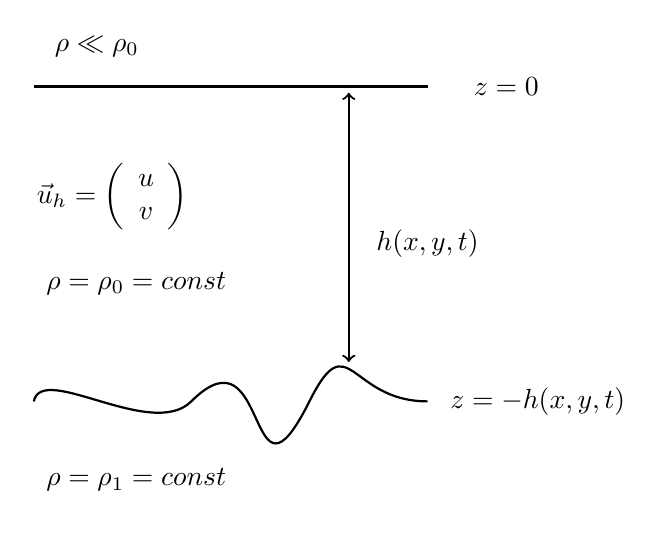
\begin{tikzpicture}
            \draw[thick] (0,0) .. controls +(0.1,0.5) and +(-0.5,-0.5) .. (2,0) .. controls +(1,1) and +(-0.8,-1.6) .. (3.5,0) .. controls +(0.5,1) and +(-1,0) .. (5,0);
            \node[] at (6.4,0) {$z=-h(x,y,t)$};
            \draw[thick] (0,4) -- (5,4);
            \node[] at (6,4) {$z=0$};
            \draw[thick,<->] (4,3.92) -- (4,0.5);
            \node[] at (5,2) {$h(x,y,t)$};
            \node[] at (1.3,1.5) {$\rho=\rho_0=const$};
            \node[] at (0.8,4.5) {$\rho \ll \rho_0$};
            \node[] at (1,2.6) {$\vec{u}_h=\left( \begin{array}{c}u\\v\end{array} \right)$};
            \node[] at (1.3,-1) {$\rho=\rho_1=const$};
        \end{tikzpicture}
        \caption{The Reduced Gravity System}
        \label{RG Fig}
    \end{figure}
\end{minipage}

Where $g'$ is the reduced gravity and is defined as follows:

\begin{fact}{The Reduced Gravity}{RG Box}\label{RG Box}
    We define the reduced gravity $g'$ as:
    \begin{align}
        \BOX{g'=\frac{\Delta \rho_0}{\rho}g}
    \end{align}
    where $g=$ is the acceleration due to the gravity; $\rho$ is the density of the layer; and $\Delta \rho = \rho_1-\rho_0$, where $\rho_0$ is the density of the layer under consideration and $\rho_1$ is the density of the underlying layer.

    The reduced gravity equations are exactly the same as the \hyperref[shallow box]{Shallow Water Equations} but with all instances of $g$ replaced with a $g'$.

    It is generally the case that $g'\ll g$. 
\end{fact}

Importantly, the reduced gravity system affects the \hyperref[SW Def Radius Box]{Rossby Deformation Radius}, now given by the following expression:
\begin{align*}
    L_d = \frac{\sqrt{g' H}}{f}
\end{align*}
Therefore, since generally $g'\ll g$, and $L_d\sim\sqrt{g'}$, then $L_d$ is much smaller than we anticipated before.

\section{Justifying the Shallow Water System}\label{SW Justification}

\chapter{3D Systems}\label{3D Systems}

\section{Gravity Waves}

\subsection{The Boussinesq Approximation}

\section{Quasi-Geostrophic Theory}

\section{Quasi-Geostrophic Rossby Waves}

\section{Instabilities and Geostrophic Turbulence}

\chapter{Ocean Circulation}\label{Oceans}

As already touched upon, the oceans, while similar to the atmosphere in the sense that it is a fluid affected by gravity (and so stratification) and rotation (and so coriolis), differs dynamically due to a few facts.

\begin{enumerate}
    \item Equation of state: $g'$ is much smaller, so $L_d$ is much smaller
    \item Rossby number
    \item External forcing
    \item Bathymetry
\end{enumerate}

We'll be exploring some effects of external forcing \ref{Ekman Transport} and the small rossby number \ref{Sverdrup Balance}.

\section{Ekman Transport}\label{Ekman Transport}

We begin by considering the effect of external forcing due to friction. For the ocean, this will be due to the atmosphere blowing over the ocean, which exerts a shear stress on the surface of the ocean, forcing the ocean to move in the same direction as the air. A \textbf{stress} is a force per unit area across a boundary. In this case, this is the boundary between the atmosphere adn the ocean. A \textbf{shear} stress is 

Actually, phenomena we discuss here is applicable to the atmosphere as well: the ground exerts a shear stress on the atmosphere in the opposite direction that the atmosphere is flowing in!

Ekman transport is the transport due to the circulation of 

Assume $Ro\ll1$ so we can neglect the acceleration/advection term in Equation \ref{Horizontal Approximate} and that $\rho=\rho_0=const$:
\begin{align*}
    f\vec{k}\times\vec{u}+\frac{1}{\rho_0}\vec{\nabla}_h p = \vec{F}_b
\end{align*}

We now no longer neglect other forces, and reintroduce the horizontal stress force. We assume that the horizontal stresses vary the most vertically, which means that we can write $F_b$ to a good approximation as follows:
\begin{align*}
    \vec{F_b} = \frac{1}{\rho_0}\frac{\partial \vec{\tau}}{\partial z}\\
    \tau=\underbrace{\rho_0\nu\frac{\partial \vec{u}_h}{\partial z}}_{\text{viscous stress}}-
    \rho_0 \vec{u}_h'w'
\end{align*}
where $\vec{\tau}$ is the horizontal stress vector\footnote{If you are familiar with fluid mechanics, you will notice that, in reality, the stress is actually a tensor.}. 

\subsection{Ekman Spiral}

\subsection{Ekman Volume Flux}

\section{Sverdrup Balance}\label{Sverdrup Balance}

\section{Stommel Box Model}\label{MOC}

In this section we aim to construct a simple box model of the \textbf{Atlantic Meridional Overturning Circulation} (AMOC). The AMOC is a complex overturning circulation, consisting of warm waters which flow from the Southern Ocean northward, before turning cold and salty, sinking in the North Atlantic, and flowing southward to complete the loop.

This is a somewhat oversimplified version of the \textbf{MOC}, but I sadly don't have the time nor energy to get into it at this point. 

Crucially, though, the water must sink in the North Atlantic, and this requires the water to be denser or at least as dense as the water below it. We must therefore consider the \textbf{equation of state} that governs the density of sea water.

The equation of state is horribly complicated, and there (to the best of my knowledge) is no theoretical way to derive it. Instead, we use an empirically found Gibbs function of seawater $G$ to calculate the equation of state. Recalling that $dG = -S\,dT + \rho\,dp+\dots$, you can see that $\rho=\partial G/\partial p$.

This, still, is too complicated for our purposes, so we simply linearise the equation of state and assume that water is incompressible (water is actually compressible).

\begin{gather}
    \rho=\rho_0(1-\alpha (T-T_0)+\beta(S-S_0))
\end{gather}